\chapter{Theory and Methods \label{chap: Methods}}


The density of states contains important physical information about the presence of zero-modes which can be caused by the Kondo effect or by a Majorana quasi-particle. Studying this quantity will allow as to observe both effects separately inside each quantum dots. In this chapter we describe the two methods that we will use during the entire project to compute the DOS:

\begin{itemize}
 \item The first method uses Zubarev's Green function formalism \cite{zubarev_double-time_1960}. This approach requires the solution of the equations of motion,  a process that we simplify introducing the graph-Gauss-Jordan elimination method (\ref{sec:GraphMethod}). In the non-interacting regime, this method allows us to obtain an exact analytical expression of this quantity for density of states of the system.

 \item Interacting systems are more complex and cannot be solved analytically. Instead, we appeal to the renown numerical renormalization group (NRG) to deal with the strong correlations of the interacting Anderson model \ref{sec:The-Numerical-Renormaliztion}. The NRG is famous for providing the most complete explanation of the Kondo effect. Know we intend to use it to study the co-existence of Kondo and Majorana physics.
\end{itemize}

Both methods will be tested on the model of a double quantum dot attached to a metallic lead. We will observe that at very low energies, the physics of interacting systems emulate characteristic features of the non-interacting model. The methods developed in this chapter will be tested  again in \ref{chap:Majorana} for a QD coupled to a Majorana chain. Finally we will use them to make our leading contribution to this theory, the analysis of a double quantum dot attached  to a Majorana wire (\ref{chap:Results}). 


\section{Green function formalism \label{sec:transport} }

The Green function $G$ of a Hamiltonian $H$ is the operator that satisfies the homogeneous equation 
\begin{equation}
    \left(i\hbar\frac{\partial}{\partial t}-H\right)G\left(t-t'\right)=\delta(t-t'). \label{eq:greeni}
\end{equation}

\noindent This type of differential equations are usually solved with a Fourier transform 
\begin{equation}
    \Green{H}=\int_{-\infty}^{\infty}\text{d}(t-t')\ G(t-t')e^{-i\omega(t-t')}.
\end{equation}

\noindent By convention we took  $\hbar =1$ so that we can unify units of frequency and energy. This turns equation \eqref{eq:greeni} into a function of the energy $\omega$ such that 
\begin{equation} 
(\omega+is -H)\Green{H}=I. 
\end{equation}
\noindent The term $+is$ in the previous Hamiltonian is part of a mathematical trick quite common in this theory. During the whole procedure, the Green function acts on the complex field, with $+is$   making reference to a small imaginary part that allows to avoid singularities in the real line. But when we need to obtain a physical interpretation, we will take the limit $s\rightarrow0$ to obtain the result for real energies. 

The next step is to decompose $\Green{H}$ in the eigenbase of the Hamiltonian $\{\ket{\alpha}\}$  by 


\begin{equation}
    \langle \alpha  \vert \Green{H}\ket{\alpha'}=\frac{\delta_{\alpha\alpha'}}{\omega - is -\ep_\alpha}=\frac{\delta_{\alpha\alpha'}(\omega + is -\ep_\alpha)}{(\omega-\epsilon_{\alpha})^{2}+s^{2}}.
\end{equation}

From the Cauchy relation            
\begin{equation}
\lim_{s\rightarrow0}\frac{s}{(\omega-\epsilon_{\alpha})^{2}+s^{2}}=\pi\delta(\omega-\epsilon_{\alpha})
\end{equation}
we obtain 
\begin{equation}
    Im \langle \alpha  \vert \Green{H}\ket{\alpha'}] = \pi \delta(\omega -\epsilon_\alpha)\delta_{\alpha,\alpha'}.
\end{equation}
Note that the sum of $Im[ \langle \alpha  \vert \Green{H}\ket{\alpha'}]$ over all the eigenstates of $H$ is simply $\pi$ times the density of states:

\begin{equation}
    \rho(\omega)=-\frac{1}{\pi} \sum_\alpha Im \left[ \langle \alpha  \vert \Green{H}\ket{\alpha'}\right] = \sum_\alpha \delta(\omega-\epsilon_\alpha) . \label{eq:DOS_def}
\end{equation}

\subsection{Green function of fermion operators and the equations of motion}

 In many body physics, fermion operators are defined by quantized fields over time satisfying anti-commutation relations , such that for any two independent operators at a time $t$ $(A(t)  , B(t))$  we have
 \begin{equation}
    \{ A(t) , B(t) \} = \delta_{B,A^\dagger} .
 \end{equation}
\noindent  Two types of Green functions are usually defined in this case.

 \begin{align}
  G^r_{A,B}(t,t') =& -i\theta(t-t')\langle \{ A(t) , B(t') \} \rangle  .  \label{eq:TempGreen}  \\
   G^a_{A,B}(t,t') =& -i\theta(t'-t)\langle \{ A(t) , B(t') \} \rangle  .
 \end{align}
  
 % \end{equation}
\noindent Where $\theta(t-t')$ is the Heaviside step function and  the brackets $\langle \rangle$ refer to the statistical mean over thermal states. $G^r_{A,B}$ is called the retarded Green function. It is non-zero only if $t>t'$, such it allows to compute the response of the system after it has been perturbed. 
 The advanced Green function $G^a_{A,B}$ is the adjoint of $G^r_{A,B}$ and represents exactly the opposite regime. 

  Usually we can obtain all relevant physical properties just with the retarded Green function, including the density of states.  To perform this, we need to take first the Fourier transform of the retarded green function to enter into the energy domain
\begin{equation}
   \Green{A,B}=\int_{-\infty}^{\infty}\text{d}(t-t')\  G^r_{A,B}(t,t')e^{-i\omega(t-t')}.
\end{equation}

 \noindent Now, in this formalism, the DOS is associated to a fermion operator $A$. Similar to  \eqref{eq:DOS_def}, it can be computed as 
\begin{equation}
    \rho_{A,A^\dagger}=-\frac{1}{\pi}Im\left[\Green{A,A^\dagger}\right].
    \label{eq:Density of States}
\end{equation}

The density of states contains important physical information related to operator $A$. In our case, operator $A^\dagger$ will be related to the dot's creation operator  $d^\dagger$. Therefore,  computing \eqref{eq:Density of States} will allow us to observe the hybridization of the dot's discrete states and the creation of other energy levels due to the interaction with the lead and other impurities. In particular, we are interested in studying the zero-modes of the system which are the main signatures of Kondo and Majorana physics. 





%  $ A(t)B(t')$ or  $B(t')A(t)$ is considered into account according to the time operation. 
%   and advanced $G^a_{A,B}$  Green functions are defined as 

%  In many body physics we use second quantization operators to define the Green functions.

%   Two given fermion operators $a_i(t)$ , $a_j(t')$ satisfy anticommutation relations of the form $\{ a_i(t) , a_j(t')\}$

%  second quantization most computations are performed with double time green functions of the form 

% \begin{equation}
% \begin{aligned}
%   G_{A,B}(t-t') =& \langle \mathbb{T}( A(t),B(t') ) \rangle. \label{eq:TempGreen} \\
%   := & \theta(t-t')  A(t),B(t') - \theta(t'-t) B(t'),A(t)
%  \\
%   =&  \theta(t-t')  A(t),B(t') - \theta(t'-t) B(t'),A(t)
% \end{aligned}
 
% \end{equation}

%   are not only associated with the Hamiltonian, but also with the fermion operators. These operators are time dependent. Then, The for two fermion operators $A$ and $B$ ,  the Green function is then defined as the mean value of the time ordered multiplication of both operators

% \begin{equation}
% \begin{aligned}
%   G_{A,B}(t-t') =& \langle \mathbb{T}( A(t),B(t') ) \rangle. \label{eq:TempGreen} \\
%   := & \theta(t-t')  A(t),B(t') - \theta(t'-t) B(t'),A(t)
%  \\
%   =&  \theta(t-t')  A(t),B(t') - \theta(t'-t) B(t'),A(t)
% \end{aligned}
 
% \end{equation}
 
But before talking more about the DOS,  we still  need an efficient method to compute the Green function of the system. We can achieve this by analyzing  the evolution of the retarded Green function in the time domain. This is determined by Schroedinger's differential equation
in the Heisenberg picture 
\begin{equation}
i\frac{dA(t)}{dt} =\left[A(t),H\right],
\end{equation}
\noindent which allows us to derive

\begin{align}
i\frac{d}{dt}G_{A,B}^{r}\left(t,t'\right)&=-i^{2}\langle\left[A(t),B(t)\right]\rangle\delta\left(t-t'\right)-i\theta\left(t-t'\right){\displaystyle \left\langle \left\{ i\frac{dA(t)}{dt},B(t')\right\} \right\rangle } \\
=& \delta_{A^{\dagger},B}\delta\left(t-t'\right)-i\theta\left(t-t'\right)\left\langle \left\{ \left[A(t),H\right],B(t')\right\} \right\rangle  \\
= & \delta_{A^{\dagger},B}\delta\left(t-t'\right)+G_{\left[A,H'\right],B}^{r}\left(t,t'\right). \label{eq:Motion}
\end{align}

When taking the Fourier transform of \eqref{eq:Motion} we obtain the following equation in the energy domain  
\begin{equation}
    \omega\Green{A,B}=\delta_{A^{\dagger},B}+\Green{\left[A,H\right],B}.
    \label{eq:Transport}
\end{equation}


\noindent In a set of operators $\{A_1, A_2, \ldots \}$ \eqref{eq:Transport} defines a system of transport equations describing the flow of state transitions of the operators in our model. This system receives the  name of equations of motion. In this thesis we will identify each set of equations with a flow graph. This will be our leading method to compute the green functions of the system.


% ----------------------------- Graph Method-----------------------
\subsection{Graph-Gauss-Jordan elimination process: Solving the equations of motion \label{sec:GraphMethod}}


Solving the transport equations involves dealing with a set of linear equations where all the possible variables including  $\omega$ , and the Hamiltonian parameters are assumed to be constant.  This can be done by  Gauss-Jordan elimination, noting that after each elimination process we need to carry on the account in terms of the initial  variables. The solution  will be a polynomial fraction.  When the number of operators in the Hamiltonian increases the number of terms in the polynomial grows-up rapidly according to the number of initial parameters. This reveals the importance of exploring new methods that could simplify the solution of this system, and present a readable factorized expression of the final solution.   \\

The method presented here uses graph theory algorithms that provide a shortcut to Gauss-Jordan elimination \cite{spielman10}. We will explain this method by solving  the transport equations for a non-interacting $(U=0)$ DQD connected to one lead. 

According to the Anderson model the Hamiltonian for this system looks like 
\begin{equation}
    H=\sum_{i=1}^2\epsilon_{i}d_{i}^{\dagger}d_{i}+ t_{dots}d_{1}^{\dagger}d_{2}+t_{dots}^*d_{2}^{\dagger}d_{1}+\sum_{k}\left(V_{i}d_{i}^{\dagger}c_{\mathbf{k}}+V_{i}^{*}c_{\mathbf{k}}^{\dagger}d_{i}\right) + \epsilon_{\mathbf{k}}c_{\mathbf{k}}^{\dagger}c_{\mathbf{k}}.
    \label{eq:HDQD}
\end{equation} 
\noindent Where the operators $d^\dagger_1$ and $d^\dagger_2$ create an electron in dots $1$ and $2$ respectively \footnote{This case is different from the Anderson model defined in \ref{sec:Anderson}, where the $d^\dagger_i$ where creation operators in distinct energy levels, not dots.}. Since the system is non-interacting, we ignore the spin-degeneracy of this Hamiltonian.   The only new parameter here is the term $t_{dots}$, which represents the tunneling between both quantum dots. 

 Using equation \eqref{eq:Transport} with $B = d_1^\dagger$ and $A$ shifting among all the other operators we compute the following  transport equations
\begin{align}
     \left(\omega-\epsilon_{1}\right)\Green{d_{1},d_{1}^{\dagger}}&=1+t_{dots}\Green{d_{2},d_{1}^{\dagger}}+V_{1}^{*}\sum_{\mathbf{k}}\Green{c_{\mathbf{k}},d_{1}^{\dagger}}, \label{eq:green1}  \\
     \left(\omega-\epsilon_{\mathbf{k}}\right)\Green{c_{\mathbf{k}},d_{1}^{\dagger}} &= V_{1}\Green{d_{1},d_{1}^{\dagger}}+V_{2}\Green{d_{2},d_{1}^{\dagger}}, \label{eq:green2} \\
     \left(\omega-\epsilon_{2}\right)\Green{d_{2},d_{1}^{\dagger}}&= t_{dots}\Green{d_{1},d_{1}^{\dagger}}+V_{2}^{*}\sum_{\mathbf{k}}\Green{c_{\mathbf{k}},d_{1}^{\dagger}}. \label{eq:green3} 
\end{align}
    %  \left(\omega-\epsilon_{1}\right)\Green{d_{1},d_{1}^{\dagger}}	= & 1+t_{dots}\Green{d_{2},d_{1}^{\dagger}}+V_{1}^{*}\sum_{\mathbf{k}}\Green{c_{\mathbf{k}},d_{1}^{\dagger}} \\

    % \left(\omega-\epsilon_{\mathbf{k}}\right)\Green{c_{\mathbf{k}},d_{1}^{\dagger}}= & V_{1}\Green{d_{1},d_{1}^{\dagger}}+V_{2}\Green{d_{2},d_{1}^{\dagger}} \\

    % \left(\omega-\epsilon_{2}\right)\Green{d_{2},d_{1}^{\dagger}}= & t_{dots}\Green{d_{1},d_{1}^{\dagger}}+V_{2}^{*}\sum_{\mathbf{k}}\Green{c_{\mathbf{k}},d_{1}^{\dagger}}. \\
 \noindent This system is already closed, hence, it will have a unique solution. The associated matrix form is  \begin{equation}
% \chapter{Motivation}
\section{Majorana Fermions}

The  Majorana Fermions, so called in the name of the Italian physicist Ettore Majorana, where first defined in the attempt to find a real solution of the Dirac equation. The real field that solves this equation $\Psi_M$ , describes a fermion which is its own antiparticle. Hence it has no electric charge nor mass.  Till these days, no fundamental particle with these characteristics has been observed. However, in the last few years, there has been a huge speculation about the possibility of finding Majorana Fermions as a quasiparticle inside certain condensed matter systems. 

One of the most famous examples of these systems is the Kitaev chain which is the main objective of the this subsection. 


\section{The Kitaev Chain}
The Kitaev chain is a toy model in tight binding that represents a  finite $p$-wave superconducting wire. The main Hamiltonian is given by 
\begin{equation}
H = \sum_{i} \left[ -t(a_i^{\dagger} a_{i+1} + a_{i+1}^{\dagger}a_i) -\mu a_i^{\dagger} a_{i} +  \Delta a_{i}a_{i+1} + \Delta^* a_{i+1}^{\dagger}a_i^{\dagger} \right].  \label{eq:kitaevHam}
\end{equation}

Where $\mu$ is the chemical potential, so that $\mu a_i^{\dagger} a_{i}$ is the energy associated to each free state. $t(a_i^{\dagger} a_{i+1} + a_{i+1}^{\dagger}a_i)$ represents the interaction between neighbouring sites which is determined by the hopping term $t$. The remaining terms describe the superconducting properties of the system as is is established by the BCS theory of superconductivity. $\Delta$ is a complex superconducting parameter with the form  $\Delta = e^{i\theta} \super$. The associated terms represent the Cooper pairs which can be created or annihilated at neighbouring sites of the system.

The form of hamiltonian \prettyref{eq:kitaevHam} favors the possibility of introducing new operators $\gammaA{j}$ and $\gammaB{j}$ such that

\begin{equation}
\gammaA{j} = e^{i\theta /2}a_j+ e^{-i\theta/2 } \ann_j \ \ , \ \ \gammaB{j} = -i(e^{i\theta /2}a_j - e^{-i\theta/2} \ann_j).
\label{eq:majoranaTrans}
\end{equation}
It is simple check that these operators are self-adjoint $(\gammaA{j}^\dagger = \gammaA{j}, \gammaA{j}^\dagger = \gammaB{j})$. This is a required constraint for the Majorana particles. In addition they satisfy the fermionic anti-commutation relations
\begin{equation}
\begin{aligned}
\{\gammaA{i}, \gammaA{j}\} = \{ & \gammaB{i} , \gammaB{j}\} = 2\delta_{ij}  ,\\ 
  \{\gammaA{i}, \gammaB{j} & \} =0.
\end{aligned} 
\label{majoranaRel}
\end{equation} 
This allows us to understand the operators $\gammaA{i} , \gammaB{i}$ as majorana fermions. If we also take the inverse of \prettyref{eq:majoranaTrans} we obtain that each  (Dirac) fermion in Hamiltonian \eqref{eq:kitaevHam} is composed by two majorana fermions such that 
$$a_j = \frac{e^{-i\theta/2}}{2}(\gammaA{j}+ i\gammaB{j})$$
We could even adventure to say that these majorana operators are actually dividing the Dirac fermions into real($\gammaA{}$) and imaginary $(\gammaB{})$ part ,the same way as complex numbers are a composite of two real numbers. 

The new Kitaev Hamiltonian in the Majorana representation looks like 

\begin{equation}
H = \frac{i}{2} \sum_{j} \left[ -\mu \gammaA{j}\gammaB{j}  + (t- \super) \gammaB{j}\gammaA{j+1} + (t+ \super) \gammaA{j}\gammaB{j+1} \right]+Const,\label{eq:HamMajorana}
\end{equation}

Depending on the values of parameters $\mu, t$ and $\super$ we can identify two regimes represented by the following situations:


%\begin{figure}[t]
%$$\includegraphics[scale=0.5]{KitaevtopPhases.jpg}
%\centering
%\label{top.phases kitaev}
%\caption{{\small \textit{Taken from \cite{bernevig2015topological}. Ilustration of the Kitaev chain for open boundary conditions in the Majorana representation. a)Represents the trivial case where the hopping and the superconducting term approaches to $0$. b) The non-trivial topological phase. The coupling is produced between Majoranas in different Dirac fermions }}}
%\end{figure}


\begin{enumerate}
\item{If $\super = t = 0, \mu <0$} Hamiltonian \eqref{eq:HamMajorana} becomes $\frac{-i\mu}{2} \sum_{j} \gammaA{j}\gammaB{j}$ which represents the coupling of the Majoranas in the same Dirac fermion. (See figure \ref{top.phases kitaev} (a))

\item{If $\super = t > 0, \mu =0$} the situation is much more interesting. The Hamiltonian \eqref{HamMajorana} takes the form $H = 2ti\sum_{j} \gammaA{j}\gammaB{j+1}$. This implies that the coupling is performed between  Majoranas of different Dirac fermions leaving the edge Majorana operators ($\gammaA{1}$ and $\gammaA{2}$) uncoupled . This produces a new degeneracy in the ground state due to the emergence of a state produced by the uncoupled Majorana operators. The new state is localized at the edges of the chain.(See figure \ref{top.phases kitaev} (b)) 
\end{enumerate}

% \chapter{Coupling the Majorana Zero Mode to a Double Quantum Dot \label{chap:Results} }
%--------------------------------------------------------------------------
\begin{figure}[hbt]
    \centering
    \includegraphics[scale=0.4]{IMAGES/GenModel.png}
    \caption{\label{fig:GenModel} Model for the DQD-Majorana system. Solid lines: Hopping interactions ($t_{dots}$: inter-dot coupling , $V_1,V_2$ couplings of QD1 and QD2 with the lead. ). Dashed lines: Majorana spin-$\dw$ effective couplings \eqref{eq:MajoranaCoupling} $t_1,t_2$. The atomic energy levels appear inside each QD $\ep_1, \ep_2$ are tuned by the gate voltages. The coulomb interaction is represented by $U_1,U_2$.  The red dashed horizontal lines represent the Fermi level. \protect \Source{ } } 
\end{figure}

\noindent The DQD-Majorana model is the most fundamental structure where Majorana manipulation is possible. Tunneling Majorana modes in this device have already inspired a few theoretical studies \cite{silva_andreev_2016,ivanov_coherent_2017} and experimental setups confirming the observations of Andreev molecules \cite{su_andreev_2017}. However, there is still no complete analysis of the transitions of the Majorana signatures between the QDs in this model, even though quantum tunneling of a MZM into a double dot offers several possibilities for MZM manipulation.  

 In this chapter, we will explore  different possibilities for Majorana manipulation in a device consisting of a DQD coupled to a MZM and a metallic lead (See \ \ref{fig:GenModel}). The simplicity of this model allows us to explore analytically different geometries of QD's from linear and symetric couplings to T-junctions (Fig.\ \ref{fig:MajoranaModels}). As in the previous models , we will consider both non-interacting and interacting regimes. 


% Tunneling of a MZM into a double dot shows several possibilities for manipulation of MZM,  there is still no complete analysis of the transitions of the Majorana signatures between the QDs in this model. 


% \noindent The idea of using Majorana islands formed by QDs coupled to topological superconducting wires has recently turned on new lights  into the fabrication of of quantum architectures \cite{barkeshli_physical_2015,karzig_scalable_2017}. The main insight  of this method is that today’s precise experimental control over the parameters of QDs -energy levels, tunneling couplings, etc.- offers the unique possibility of manipulating the Majorana modes inside multi-dot systems. The simplest case where Majorana manipulation is possible is in a double quantum dot. So far, no complete analysis of this basis case has been done. The purpose of this chapter is to fill this gap by realizing a full quantum transport study of the effects of coupling a Majorana mode with a double quantum dot. For this, we combine the ballistic transport and the NRG approach developed in \ref{chap: Methods}. 


% As previously stated in the , Majorana-QD  architectures turn on new lights to the area of topological quantum computing. 



% Using the ideas from the previous chapters we are going to test if it is possible to manipulate the Majorana zero mode in the double quantum dot.  

% In the previous chapter we observed the result of coupling a Majorana mode to a quantum dot. The Majorana signature characterized by a decay of the Fermi peak to the half of its original height is a



 The model in \ref{fig:GenModel} can be described from the combination of the Hamiltonians of a QD-Majorana system \eqref{eq:QD-Mham} and a DQD \eqref{eq:HDQD}. Integrating these models we obtain

\begin{equation}
H =\sum_{i=1}^2\sum_{k,\sigma}\left(\epsilon_{i}+\frac{U_i}{2}\right)d_{i\sigma}^{\dagger}d_{i\sigma}+ \frac{U_i}{2}(d_{i \sigma}^{\dagger}d_{i \sigma}-1)^{2} + t_i\gamma d_{i,\dw} + V_id^\dagger_{i\sigma}c_{k\sigma}+ t_{d o t s}d_{1 \sigma}^{\dagger} d_{2 \sigma} +\text{h.c}.
\label{eq:Generalmodel}
\end{equation}

Where $V_1,V_2$ is the coupling of dots $1,2$ to the lead. $t_1,t_2$ define the Majorana couplings with each dot. $t_{dots}$ is the inter-dot coupling. $\ep_1,\ep_2$ are the energy levels of the dot, which are tuned by the the gate voltage and $U_1,U_2$ are the coulomb repulsion parameters. 
% \Jesus{I neglected $\epsilon_M$ in this case. Depending on the future NRG results I will choose to add it or leave it that way. }



\section{Applying our methods to the DQD-Majorana system}


% In order to understand the physical properties of this model, we probed a set of thought processes. The main variable in this analysis is the density of states.  We  will observe its evolution on both QDs under the tuning of the model parameters such as the majorana couplings ($t_1 , t_2$)  ,  gate voltages ($\ed{1} , \ed{2} $) and the inter dot coupling ($t_{dots}$). With these processes intend to show whether it is possible to "manipulate" the majorana modes inside the dots by tuning the established parameters. The number of possible combinations of parameters is huge and not all of them lead to important results. So on, we used the ballistic transport to select which arrangements could bring novel results. The most interesting models were simulated with NRG in the interacting case \ref{fig:MajoranaModels}.  

\subsection{Non-interacting Green function:}

%  To solve the transport equations using the graph method from \ref{sec:GraphMethod} first not that 
This new model is a combination between the DQD  (\ref{fig:graphDQD}) and the Majorana-QD  \ref{fig:green-M-QD}(b). We can use the trick in \ref{sec:GreenMaj-DQD} to get rid of the Green function $\Green{f_\dw,d^\dagger_1}$ for the second Majorana operator. This allows us to obtain the following transport equations 
 
 
 
%  As we did previously in \ref{sec:GreenMaj-DQD} the transport equations for $f_\dw$ and $f^\dagger_\dw$ are 
% \begin{align}
%         \left(\omega-\epsilon_{M}\right)\Green{f_{\downarrow},d_{1\downarrow}^{\dagger}}&=\frac{t}{\sqrt{2}}\left(\Green{d_{1\downarrow},d_{1\downarrow}^{\dagger}}-\Green{d_{1\downarrow}^{\dagger},d_{1\downarrow}^{\dagger}}\right) \\
%     \left(\omega+\epsilon_{M}\right)\Green{f_{\downarrow}^{\dagger},d_{1\downarrow}^{\dagger}}&=\frac{t}{\sqrt{2}}\left(\Green{d_{1\downarrow},d_{1\downarrow}^{\dagger}}-\Green{d_{1\downarrow}^{\dagger},d_{1\downarrow}^{\dagger}}\right),
% \end{align}
% \noindent which allows us to take $\Green{f_{\downarrow}^{\dagger},d_{1\downarrow}^{\dagger}} = \frac{\omega + \epsilon}{\omega -\epsilon}\Green{f_{\downarrow}^{\dagger},d_{1\downarrow}^{\dagger}} $. Therefore, we can eliminate $\Green{f_{\downarrow}^{\dagger},d_{1\downarrow}^{\dagger}} $ from the equations even before we start Gauss-Jordan process.
 
 \begin{equation}
     \left[\begin{array}{ccccccc}
\omega-\epsilon_{1} & -V_{1}^{*} & -t_{dots} & -T_{1} & 0 & 0 & 0\\
-V_{1} & \omega-\epsilon_{k} & -V_{2} & 0 & 0 & 0 & 0\\
-t_{dots}^{*} & -V_{2}^{*} & \omega-\epsilon_{2} & -T_{2} & 0 & 0 & 0\\
-T_{1}^{*} & 0 & -T_{2}^{*} & \omega-\epsilon_{M} & T_{2}^{*} & 0 & -T_{1}\\
0 & 0 & 0 & T_{2} & \omega+\epsilon_{2} & V_{2}^{*} & t_{dots}^{*}\\
0 & 0 & 0 & 0 & V_{2} & \omega+\epsilon_{k} & V_{1}\\
0 & 0 & 0 & T_{1} & t_{dots} & V_{1}^{*} & \omega+\epsilon_{1}
\end{array}\right]\left[\begin{array}{c}
\Green{d_{\mathbf{1\downarrow}},d_{1\downarrow}^{\dagger}}\\
\Green{c_{k\downarrow},d_{1\downarrow}^{\dagger}}\\
\Green{d_{2\downarrow},d_{1\downarrow}^{\dagger}}\\
\Green{f_{\downarrow},d_{1\downarrow}^{\dagger}}\\
\Green{d_{2\downarrow}^{\dagger},d_{1\downarrow}^{\dagger}}\\
\Green{c_{k\downarrow}^{\dagger},d_{1\downarrow}^{\dagger}}\\
\Green{d_{1\downarrow}^{\dagger},d_{1\downarrow}^{\dagger}}
\end{array}\right]=\left[\begin{array}{c}
0\\
0\\
0\\
0\\
0\\
0\\
1
\end{array}\right],
 \end{equation}
 
 where $T_i = \frac{t_i}{\sqrt{\omega+\epsilon_M}}$. 
 
 
% ------------------------FIGURE GRAPH--------------------
     \begin{figure}[bt]
    \centering
    \includegraphics[scale=0.4]{IMAGES/Graphs/FinalGraph.png}
    \caption{\label{fig:Graph-MDQD} Graph method applied to a DQD coupled to a Majorana zero mode. a) Initial stage. b) Eliminated vertexes $c^\dagger_k$, $c_k$, $d_{2, \downarrow}$ , $d^\dagger_{2, \downarrow}$ in that order. c) Eliminated vertexes $d^\dagger_{1, \downarrow}$ and $f_\dw$, the final energy is $\omega-\Green{d_1,d_1^\dagger}$  . \protect\Source{   }} 
    \end{figure}

% ------------------------FIGURE GRAPH---------------------------
 The graph representing this equation is in  \ref{fig:Graph-MDQD}(a). Using the algorithm in \ref{sec:Algorithm} we start eliminating vertexes $c_k,c^\dagger_k, d_{2,\dw}$ and $ d^\dagger_{2,\dw}$ in that order. The self-energies associated to $d_{1,\dw}$ and $d^\dagger_{1,\dw}$ will be similar to the energy of the DQD \eqref{eq:EnDQD} giving 
\begin{equation}
    \epsilon_{DQD}^{\pm}=\pm\epsilon_{1}+\sum_{\mathbf{k}}\frac{V_{1}V_{1}^{*}}{\omega-\epsilon_{\mathbf{k}}}+\frac{\left\Vert \pm t_{dots}+\sum_{\mathbf{k}}\frac{V_{1}V_{2}^{*}}{\omega-\epsilon_{\mathbf{k}}}\right\Vert ^{2}}{\omega\mp\epsilon_{2}-\sum_{\mathbf{k}}\frac{V_{2}V_{2}^{*}}{\omega-\epsilon_{\mathbf{k}}}}. \label{eq:epDQD}
\end{equation}
\noindent There is also a correction in the couplings between the Majorana mode and $d_{1,\dw}$, $d^\dagger_{1,\dw}$ given by 

\begin{equation}
    T_{\pm}=\pm t_{1}\pm t_{2}\frac{\left(\pm t_{dots}+\sum_{\mathbf{k}}\frac{V_{1}V_{2}^{*}}{\omega-\epsilon_{\mathbf{k}}}\right)}{\omega\mp\epsilon_{2}-\sum_{\mathbf{k}}\frac{V_{2}V_{2}^{*}}{\omega-\epsilon_{\mathbf{k}}}}. \label{eq:T+-}
\end{equation}

\noindent In addition, since the Majorana is in contact with dot $2$, there is an extra-term appearing in the  Majorana self-energy given by 
\begin{equation}
    \epsilon_{M2}=\omega-\epsilon_{M}-\frac{\frac{\omega}{\omega+\epsilon_{M}}\left\Vert t_{2}\right\Vert ^{2} } {\omega-\epsilon_{2}-\sum_{\mathbf{k}}\frac{V_{2}V_{2}^{*}}{\omega-\epsilon_{\mathbf{k}}}}-\frac{\frac{\omega}{\omega+\epsilon_{M}}\left\Vert t_{2}\right\Vert ^{2}}{\omega+\epsilon_{2}-\sum_{\mathbf{k}}\frac{V_{2}V_{2}^{*}}{\omega+\epsilon_{\mathbf{k}}}}. \label{eq:M2}
\end{equation}
It only remains to eliminate out vertexes $d^\dagger_1$ and $f_\dw$  to obtain the green function 

\begin{equation}
    G_{{d_{1\downarrow},d_{1\downarrow}^{\dagger}}}\left(\omega\right)=\frac{1}{\omega-\epsilon_{DQD}^{+}-\frac{\left\Vert T_{+}\right\Vert ^{2}}{\omega-\epsilon_{M2}-\frac{\left\Vert T_{-}\right\Vert ^{2}}{\epsilon_{DQD}^{-}}}}.
    \label{eq:Green_NonInteracting}
\end{equation}

This simple formula summarizes the transport information through the first dot of the non-interacting Majorana-DQD system.  To compute the DOS we just need to replace  $\sum \frac{V_iV^*_i}{\omega -\epsilon_k}= -i\Gamma_i$ as performed in \ref{sec:GraphMethod}. By plotting the final DOS in Mathematica we were able to observe the transitions of the Majorana mode under manipulation of the model parameters.  


\subsection{NRG for the interacting system}

The Numerical Renormalization Group (NRG) technique described in \ref{sec:The-Numerical-Renormaliztion} is the most successful methods to study interacting quantum impurity models. In this model, the impurity is described by the DQD attached to the MZM. In our code, we set a Coulomb repulsion factor of $U =17.3\Gamma_1$ in both dots and a cut-off energy of $D=2U=34.6\Gamma_1$. The spacing with other energy levels is assumed to be higher than $D$, such that only the two coulomb states are relevant for the system dynamics.  When  $\epsilon_i = \frac{U}{2}$ in both dots, the system is in the Particle-Hole-Symmetric region. At this point, each dot has an odd number of electrons, hence, at sufficiently low temperature the system will exhibit characteristic Kondo peaks at the Fermi energy \cite{wilson_renormalization_1975}. The coexistence of Kondo and Majorana zero modes is still a point of contention in the area that has never been studied in DQDs and one of the objectives of this part of the project.


% Observing how the Kondo-effect interacts with the Majorana signature in the double quantum dot is also an insight of this project. 


To  improve the efficiency of the code we used the symmetries of the system to maintain a block structure during NRG's iterative diagonalization process. This model preserves the spin-$\up$ particle number $\hat{N}_\up$ and the spin-$\dw$ parity $\hat{P}_\dw = \pm $ ($+$ even, $-$ odd). The spin-$\dw$ particle number is not preserved due to superconducting-type Majorana coupling  \eqref{eq:MajoranaCoupling} . The initial Hamiltonian is organized in blocks according to these symmetries. This block structure is preserved during the entire iteration process \cite{bulla_numerical_2008}. To compute the spectral functions, we use the density matrix renormalization group (DM-NRG) described in \ref{subsec:DM-NRG} in combination with the Z-trick method \cite{oliveira_generalized_1994}, which improves spectral resolution at high energies.


To initialize the model in \ref{fig:Code} we set $H_{-1}$ equal to 
\begin{equation}
H_{-1} =\sum_{i=1}^2\sum_{k,\sigma}\left(\epsilon_{i}+\frac{U_i}{2}\right)d_{i\sigma}^{\dagger}d_{i\sigma}+ \frac{U_i}{2}(d_{i \sigma}^{\dagger}d_{i \sigma}-1)^{2} + t_i(\gamma d_{i,\dw}+d^\dagger_{i,\dw}\gamma)+t_{d o t s}\left(d_{1 \sigma}^{\dagger} d_{2 \sigma}+d_{2 \sigma}^{\dagger} d_{1 \sigma}\right),
\label{eq:imp_Ham}
\end{equation} 
\noindent and wrote the Hamiltonian in the symmetry-block diagonal representation (see \ref{sec:Double-Dot-Majorana-Hamiltonian.}). We also include manually the Hamiltonian $H_0$ into the code (See \ref{fig:Code}) to guarantee that both quantum dots are coupled to the first site of the chain. After this, the code follows the standard NRG algorithm and prints the density matrices to initialize DM-NRG. The final result is the spectral density which contains sufficient physical information to study the MZM-DQD model. In the following section, we show how the density of states can be used to simulate the Manipulation process of an MZM inside the DQD. 




\section{Manipulation of Majorana zero modes}


\begin{figure}[bt]
\centering
\includegraphics[scale=0.7]{IMAGES/DQD-M/3Model.png}
\caption{\label{fig:MajoranaModels}. \protect\Source{}} 
\end{figure}


The density of states provides significant information about the presence of a Majorana zero modes in the dot. We characterize the Majorana signature by a robust zero-mode with two possible heights:
 \begin{itemize}
         \item \textbf{Type I: }  The spin-$\dw$ DOS is the half of the spin-$\up$ DOS  at the Fermi energy $(\rho_\dw(0)=\rho_\up(0))$. 
         \item \textbf{Type II: } A spin-$\dw$ zero mode of height $ \rho_\dw(0) = \frac{0.5}{\pi  \Gamma_1}$. 
     \end{itemize}
In our results we observe several times these two types of signatures. Type I often appears when there is a zero-mode in the spin-$\up$ DOS, which is caused by the Kondo effect in the interacting case. Type II emerges in the remaining situations. 

We call MZM manipulation to the "movements" attributed to the Majorana signature under the tunning of the dot gate voltages $( \epsilon_1 , \epsilon_2 )$. This manipulation process is performed in three different set ups that are presented in \ref{fig:MajoranaModels} with definite values of $\Gamma_2$, $t_{dots}$, $t_1$ and $t_2$. In configuration (a), we coupled the QD symmetrically to the lead and the Majorana mode. With this setup we expect to break the localization of the MZM which should split and tunnel into both dots. In setups (b) and (c) we coupled the second dot indirectly through the first dot. Hence, quantum  interference should split the zero mode in two states. Our objective is to observe what occurs with the Majorana signature in this situation. There are two options to connect the MZM in this situation. Attached it directly through the first dot (b) or indirectly through the second dot (c). Both alternatives are geometrically distinct since (b) suggests a T-junction coupling while (c) reflects a connection  in series of both QD's between the lead and the MZM. 


 %-----------F I G U R E  t1 = t2 ------
\begin{figure}[H]
    \begin{center}
    \includegraphics[scale=0.36]{IMAGES/GreenResults/t1=t2.png}
    \caption{ \label{fig:t1=t2}  Non-interacting DOS in the symmetric coupling(\ref{fig:MajoranaModels}(a)) at each QD. First column: Dot 1. Second column: Dot 2. The gate voltages vary at each row.  First row: Zero-bias in both dots $\ep_1=\ep_2=0$. Second row: $\ep_1=5\Gamma_1, \ \ep_2 =0$.  Third row: $\ep_1=0, \ \ep_2 =-5\Gamma_1$.  Bold blue lines: Spin-$\up$ DOS. Thin red lines: Spin-$\dw$ DOS. The insets at the right show which dot carries a Majorana signature, represented by a red dashed circle. Upper: First dot. Lower: Second dot. \protect\Source{}
    }
    %
    \end{center}
\end{figure}
%-----------F I G U R E  t1 = t2 ------

\subsection{Non-interacting manipulation}

 The non-interacting results for setups (a),(b) and (c) of \ref{fig:MajoranaModels} are shown at figures \ref{fig:t1=t2}, \ref{fig:t1>0} and \ref{fig:t2>0} respectively. Each figure depicts the DOS of dot $1$(left) and dot $2$(right). The gate voltage is initially $0$ in both dots at the first row. In the second row, the gate voltage is turned on to  $\epsilon_1 = 5\Gamma_1$ , while the second dot remains at $\epsilon_2 = 0$ . In the third row the first dot's voltage is off $\epsilon_1=0$ and we switch on the second dot with a negative voltage of $\epsilon_2 = -5\Gamma_1$. The inset figures at the right side of each row show which dots exhibit Majorana signatures, depicted by a red dashed circle inside the dot. These images will continuously change under the tuning of gate voltages which represents the manipulation of the Majorana signature.



In \ref{fig:t1=t2} we observe the results for the symmetric coupling setup \ref{fig:MajoranaModels}(a). In the particle hole symmetric case (first row) the DOS is equal in both dots. Note that the spin-$\dw$ (Thin red line) DOS is the half of the spin-$\up$ (Bold blue line) DOS at the Fermi energy $(\rho_\dw(0) = \frac{1}{2}\rho_\up(0))$. This type II Majorana signature is similar to the one observed when a single dot is coupled to a Majorana mode. \cite{liu_detecting_2011} We may conclude that the Majorana in tunneling inside both dots breaking the localization of the MZM. If a positive or negative gate voltage is induced in one of the dots, as shown in the second and third row of \ref{fig:t1=t2}(c)-(f),  the Majorana zero mode vanishes from that dot. Meanwhile the density of states in the other dot increases while preserving the Majorana signature. This means that the MZM is actually being induced to "leave" this dot and leak into the other by the biased voltage. This is the  first example of MZM manipulation. 


 %-----------F I G U R E  t1 >0 ------
\begin{figure}[bt]
    \begin{center}
    \includegraphics[scale=0.36]{IMAGES/GreenResults/t1>0.png}
    \caption{  \label{fig:t1>0} Non-interacting DOS of the T-dot coupling \ref{fig:MajoranaModels}(b). (b). First line (a),(b): $\ep_1=\ep_2=0$. Second line (c),(d): $\ep_1=5\Gamma_1$ , $\ep_2=0$. Third line (e),(f): $\ep_2=-5\Gamma_1$ , $\ep_1=0$.   Blue bold lines: Spin-$\up$ DOS. Red thin lines: Spin-$\dw$ DOS. The inset at the upper-right corner of each line indicates which dots  exhibit  Majorana signature, which is represented by a red dashed circle inside the dot. \protect\Source{}
    }
    %
    \end{center}
\end{figure}
%-----------F I G U R E  t1 >0 ------

Another example can  occur when the second dot is not directly connected to the lead. In this case, the inter-dot tunneling generates quantum interference which finally destroys the central peak as observed in \ref{fig:t1>0}(a) at the spin-$\up$ DOS . The spin-$\dw$ channel at \ref{fig:t1>0}(a), which is coupled to the MZM, does not exhibit the characteristic Fermi peak either. Instead, the one half Majorana signature at the Fermi energy $(\rho_\dw(0) = \frac{1}{2}\rho_\up(0))$ appears clearly inside the second dot \ref{fig:t1>0}(b). This situation prevails when the first dot's gate voltage is turned on \ref{fig:t1>0}(c)\&(d). While the first dot does not seem to exhibit any type of Majorana signature, the second dot's spin-$\dw$ DOS exhibits a robust zero-mode of height $\frac{0.5}{\pi \Gamma}$. The results are more exciting when the second dot's gate voltage is turned on in \ref{fig:t1>0}(e)\&(f). These figures clearly show how the MZM, previously localized at the second dot, is induced to leave this dot and to return into the first dot. Moreover, the DOS of spin-$\up$ and spin-$\dw$ channels are very similar to the spectral densities observed at \ref{fig:t1=t2}(d)(e), which means that the previous interference pattern has disappeared due to this gate voltage. 

 %-----------F I G U R E  t2 >0 ------
\begin{figure}[bt]
    \begin{center}
    \includegraphics[scale=0.45]{IMAGES/GreenResults/t2>0.png}
    \caption{  \label{fig:t2>0}  Non-interacting DOS of the set up in \ref{fig:MajoranaModels}(c).  First line (a),(b): $\ep_1=\ep_2=0$. Second line (c),(d): $\ep_1=5\Gamma_1$ , $\ep_2=0$. Third line (e),(f): $\ep_2=-5\Gamma_1$ , $\ep_1=0$.   Blue bold lines: Spin-$\up$ DOS. Red thin lines: Spin-$\dw$ DOS. The inset at the upper-right corner of each line indicates which dots  exhibit  Majorana signature, which is represented by a red dashed circle inside the dot. \protect\Source{}
    }
    %
    
    \end{center}
\end{figure}
%-----------F I G U R E  t2 >0 ------


The results of the third configuration \ref{fig:MajoranaModels}(c) appear in \ref{fig:t2>0}. Contrary to what was observed in the previous case, this time the Majorana signature is not destroyed by the interference but instead, the  $\frac{0.5}{\pi \Gamma}$-height MZM emerges indirectly in the first dot. This is a perfect way to separate the Majorana's spin-$\dw$ DOS from the central spin-$\up$ zero-mode which is still destroyed by the interference. In addition, the second dot still exhibits a type I Majorana signature as observed in \ref{fig:t2>0}(b). In the second row we observe that turning on the gate voltage in dot $1$  destroys the Majorana signature in both dots \ref{fig:t2>0}(c)(d). On the other hand, if the second dot's voltage is switched both dots will preserve their Majorana signature (QD1:type I, QD2: type II), while the spin-$\up$ quantum interference vanishes in the first dot.






% In this part we will discuss the three models in figure \ref{fig:Models} which are particularly interesting for the exotic behavior of their Majorana signature. The parameters $(t_1,t_2, t_dots)$ are fixed in these three models and we will take $\ep_1$ and $\ep_2$ as variables. The first model(a), represents a symmetric coupling of the DQD with the lead and the Majorana mode. In models (b) and (c) the second dot is indirectly coupled to the system through the first dot. As already analyzed in \ref{sec:GreedDQD}, the quantum interference generated by this coupling will destroy the central peak. The Majorana fermion can be either connected to the first dot (b) or to the second dot (c). The system will exhibit different Majorana signatures depending on which dot is connected to the Majorana zero mode.   



% On each case we observe three different situations. 
% \begin{itemize}
%     \item First Row: Zero bias. No gate $\ep_1 =\ep_2 = 0$.
%     \item Second Row: We turn on the first dot's gate voltage $\ep_1 = 5\Gamma_1, \ep_2 = 0$.
%     \item Third Row: We turn on the second dot's gate voltage $\ep_2 = -5\Gamma_1, \ep_1 = 0$.
% \end{itemize}

    

%     The density of states for the setup in \ref{fig:Models}.(a) is shown in Figure \ref{fig:SymCoupling}. Since the model is non-interacting, spin-$\up$ and spin-$\dw$ models are independent. The spin-$\dw$ DOS (dashed line) shows the effects caused by the Majorana zero-mode in comparison with the spin-$\up$  results (solid line). In the particle hole symmetric (first line) the DOS is equal in both dots. Note that that the spin-$\dw$ DOS is the half of the spin-$DOS$ at the fermi energy $\rho_\dw(0) = \rho_\up(0)$. This Majorana signature is similar to the one observed in the single dot case \cite{liu_detecting_2011}. We may conclude that the Majorana tunnels inside both dots. If a positive or negative gate voltage is induced in one of the dots, as shown in the second and third row of Figure \ref{fig:SymCoupling},  the Majorana zero mode vanishes. Looking to the other dot we can also observe that the Majorana signature in the other dot recovers the form observed in the single dot-Majorana model. Thus, by activating the gate voltage in one of the dots it is possible to induce the majorana mode to leave to the other dot.  

    
     
%     If the second dot is not directly connected to the lead the induced tunneling between both dots generates a path difference that destroys the central peak (See FIG\ref{fig:Interference} spin-$\up$ line). We can then proceed to connect the Majorana to each one of these dots. \ref{fig:Interference} shows the results of connecting the MZM to the first dot. Note that at zero-bias, quantum interference  destroys the Majorana mode in the first dot. However, in the second dot the spin-$\dw$ DOS is the half of the spin-$\up$ DOS at the Fermi energy, which is a clear Majorana signature. Hence, in this kind of arrangement the Majorana mode is allocated in the second dot.  \ref{fig:Interference}(e),(f) show that it is possible to reestablish the initial Majorana signature in the first dot by applying a gate voltage to the second dot. On the other hand, turning on the first dot's gate voltage does not lead to a meaningful change in the Majorana signature \ref{fig:Interference}(c),(d). While the spin-$\dw$ DOS in the first dot is still $0$ at the Fermi energy, the second dot shows a $0.5$-height zero mode. Although the spin-$\up$ DOS does not double the density of states any more, this signal is robust and equal in height to a Majorana signature which supports our claim that it is indeed a Majorana mode. 
%     If the Majorana mode is connected to the first dot, this interference will destroy the Majorana signature in the first dot. Interestingly, it is possible to observe a clear Majorana signature in the second dot characterized by a half central peak in the spin-$dw$ DOS. While turning on the first dot gate voltage seems to destroy this Majorana signature, tuning the second dots gate voltage returns the Majorana signature to the first dot. 


%     We now get into the final case that is when the Majorana mode is coupled to the second dot which is indirectly attached to the lead through the first dot. In this case \ref{fig:IndirectCoupling}(a)(b) shows that the Majorana signature is present in both dots, despite the Majorana is not directly coupled to the first dot. Moreover, we can observe that the spin-$\dw$ DOS is equal to $0.5$ at the Fermi energy while the spin-$\up$ peak has been destroyed by the interference. After turning on the first gate voltage we observe that the Majorana signature is destroyed in both dots \ref{fig:IndirectCoupling}(c)(d). This is totally opposite the results of increasing the second dot voltage which creates an stable $0.5$ Majorana signature at the Fermi energy of both dots \ref{fig:IndirectCoupling}(e)(f). 






\subsection{Interacting manipulation \label{sec:DQD-M-Interacting}}

 %-----------F I G U R E  t1=t2 ------
\begin{figure}[bt]
    \begin{center}
    \includegraphics[scale=0.52]{IMAGES/NRG/NRG-t1=t2.png}
    \caption{  \label{fig:NRG_Majorana}    Density of states of both dots in the symmetric coupling without gate voltages between the Majorana and the interacting DQD. Bold blue lines: Spin-$\up$ DOS. Thin red lines: Spin-$\dw$ DOS. Inset: Low-energy DOS.\protect\Source{}
    }
    %
    \end{center}
\end{figure}
%-----------F I G U R E  t1 =t2 ------

Now we consider a Coulomb repulsion energy of $U = 17\Gamma_1$ in both dots. The factor $ \frac{U_i}{2}(\sum_{\sigma} \hat{n}_{i\sigma}-1)^{2}$ in \eqref{eq:Generalmodel} favors states with an odd number of electrons (and holes). In addition, particle-hole equilibrium is now achieved when $\Delta \epsilon_{i} := \left(\epsilon_{i}+\frac{U_i}{2}\right)$.  Any induced gate voltage must be considered as a shifting $\Delta \epsilon_{i}$ from this equilibrium point. \ref{fig:NRG_Majorana} shows the DOS of both QDs for the symmetric coupling configuration \ref{fig:MajoranaModels}. The two peaks appearing at around $8.6\Gamma_1 = \frac{U_i}{2}$ represent the two energy levels spaced by the Coulomb repulsion factor $U$. The central spin-$\up$ peak is a consequence of the Kondo effect, \cite{hewson_kondo_1997,wilson_renormalization_1975}  while the two satellite peaks observed in the inset  are the result of the  RKKY indirect interaction between both dots.  \cite{ruderman_indirect_1954,kasuya_theory_1956,yosida_magnetic_1957} Moreover, the system presents a Majorana signature characterized by half spin-$\dw$ DOS at the Fermi energy $(\rho_\dw(0) = \frac{1}{2}\rho_\up(0))$  . Note, that in this case the Majorana signature coexists with the Kondo effect in the DQD as already predicted by Ruiz-Tijerina \textit{et al.} for a single dot. \cite{ruiz-tijerina_interaction_2015}


% If the two dots are interacting, with $U = 17.6\Gamma_1$, the spin-$\up$ density of states for the symmetric configuration (\ref{fig:Models}.(a)) is pretty similar to the DQD-symmetric model. The height of the central peak decays to $0.25$ and two new peaks appear corresponding to the dots anti-ferromagnetic interaction. In the spin-$\dw$ channel we can observe a zero mode with height equal to the half of the spin-$\up$ DOS. The effect of the Majorana coupling can be observed better on \ref{fig:2D/Shift_t1=t2}. 

\begin{figure}[H]
    \centering
    \includegraphics[scale=0.5]{IMAGES/NRG/FullEd2.png}
    \caption{\label{fig:ed2/Fermi} (a)-(d) Dependence of the density of states of setup in \ref{fig:MajoranaModels}(a) over $\omega$ and the gate voltage $\Delta \epsilon_2$ . $\Delta \epsilon_1=0$  Up: Dot 1. Down: Dot 2. Left: Spin-$\up$. Right: Spin-$\dw$.  (e) Evolution of the relation $\frac{\rho_\up(0)}{\rho_\up(0)}$ for both QDs. While QD2 losses rapidly the Majorana signature, QD1 maintains it till $\Delta \ed{2}\sim 5$. \protect\Source{}}
\end{figure}



    In this part of the project we are interested in the physics at low energy scales $\omega \sim \Gamma_1 $ close to the Kondo and MZM temperature \footnote{The MZM temperature $T_M$ can be defined by the energy scale $k_BT_M$ where the Majorana signature is visible. This effect has been plentifully discussed in a previous paper , together with its relationship with the Kondo temperature \cite{ruiz-tijerina_interaction_2015}. In the regime we are presenting in this thesis, the Majorana and Kondo temperature are similar, hence we are at an energy range where we can observe both effects co-existing. We will present further discussion about this idea in our DQD-Majorana model in a future paper.}. At this scale we can observe similar Majorana signatures compared with the non-interacting case. For instance, the inset \ref{fig:NRG_Majorana} shows the NRG results for the symmetric setup in \ref{fig:MajoranaModels}(a). In agreement with the non-interacting results, both dots have type I Majorana signatures. 

    When the gate voltage is turned on, we observe the number of holes $(\omega>0)$ increasing in the spin-$\up$, while the particles $(\omega<0)$ increase in the spin-$\dw$ (See \ref{fig:ed2/Fermi}(a)-(d) ). At $\Delta\epsilon_2 \approx 6\Gamma_1$, the Coulomb peak overlaps with the Fermi energy in the spin-$\downarrow$ channel, destroying the Majorana zero mode. This event is visible in \ref{fig:ed2/Fermi}(e), where the type one Majorana signature is clearly destroyed in Dot $1$ after $\Delta\epsilon_2 > 6\Gamma_1$. For $\Delta\epsilon_2 < 6\Gamma_1$ we observe an stable Majorana signature in dot $1$ with $\rho_\dw(0) \approx \frac{1}{2}\rho_\up(0))$. In the second dot the zero modes are absorbed by the dot, which slowly destroys the Majorana signature. 

     %-----------F I G U R E  7 ------
\begin{figure}[bt]
\begin{center}
\includegraphics[scale=0.5]{IMAGES/NRG/t1=t2.png}
\caption{ \label{fig:Nt1=t2} The same as in \ref{fig:t1=t2} for the  interacting DOS in the symmetric coupling  (\ref{fig:MajoranaModels}.\protect\Source{}
}
%
\end{center}
\end{figure}
%-----------E N D  F I G U R E  7 ------

    The red cuts in \ref{fig:ed2/Fermi} are plotted in \ref{fig:Nt1=t2} where we depict the results of Majorana manipulation. In agreement with the non-interacting case, the particle hole symmetric model receives both Majorana modes. Whenever a gate voltage is switched on, the Majorana is forced to tunnel into the other dot. We observe similar results for positive and negative gate voltages. 

 
 In the T-dot coupling \ref{fig:MajoranaModels}(b), the spin-$\up$ Kondo peak in  \ref{fig:Nt1>0} is destroyed by interference just as in the non-interacting case. This phenomenon had already been predicted for a T-junction of a double quantum dot attached to metallic leads \cite{dias_da_silva_transmission_2008}. The insight of our model is that an attached MZM should also disappear due to the same interference. Furthermore, a type I Majorana signature can be observed at very low energies in the inset of \ref{fig:Nt1>0}(b). However we have to recognize that both zero-modes decay significantly in the second dot. When the first voltage is turned on, the Majorana mode jumps onto the first dot which presents a type I Majorana signature. This is a clear difference with the non-interacting results where the Majorana signature stayed in the second dot.  If the second dot is switched on , a type II Majorana signature appears at very low energies in dot 1, which is coherent with the idea that the Majorana interference should disappear in this case. In \ref{fig:Nt1>0}(e) we identify emergence of a Fano resonance at the Fermi energy causing the sharp-asymmetric peak at $\omega = 0$. Fano resonances have already been documented in similar models in \cite{schuray_fano_2017}. We are going to talk more about this resonance in following section. 



 %-----------F I G U R E  4 ------
\begin{figure}[bt]
\begin{center}
\includegraphics[scale=0.4]{IMAGES/NRG/t1>0.png}
\caption{  \label{fig:Nt1>0} The same as in \ref{fig:t1=t2} for the  interacting DOS of the T-dot junction \ref{fig:MajoranaModels}(b). Inset in b): Zoom to low-energy DOS. \protect\Source{}
}
%
\end{center}
\end{figure}

\begin{figure}[H]
    \centering
    \includegraphics[scale=0.4]{IMAGES/NRG/c)LogEv-ed1.png}
    \caption{\label{fig:logc}  Logarithmic dependence of the density of states for interacting dots coupled in series  \ref{fig:MajoranaModels}(c) over $\omega$ and the gate voltage $\Delta \epsilon_1$. $\Delta \epsilon_2=0$. The dependence over $\Delta \epsilon_2$ produces similar results. \protect\Source{}}
\end{figure}



% -------------------FIGURES EVOLUTION ED--------------------
% \begin{figure}[h]
% \centering
% 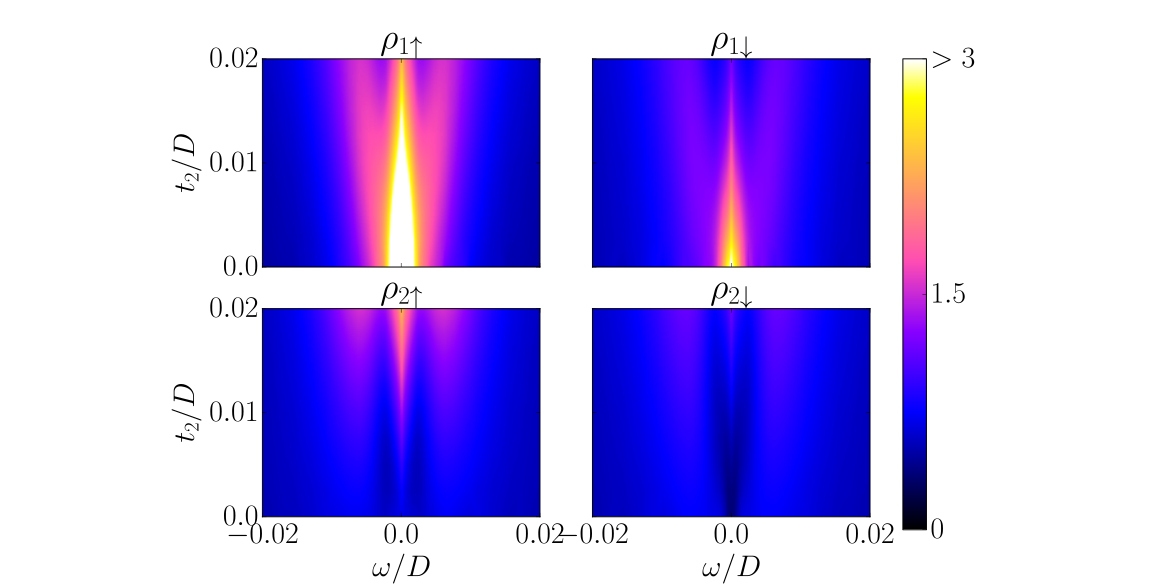
\includegraphics[scale=0.35]{IMAGES/ed2/2D.png}
% \caption{\label{fig:2D/Shift_ed2} Evolution of the DOS of both QDs through the $\ed{2}$ tuning. UP: QD1. DOWN: QD2. LEFT: Spin $\up$. RIGHT: Spin $\dw$.}
% \end{figure}



% -------------------FIGURES EVOLUTION ED--------------------


%-----------E N D  F I G U R E  4 ------
\begin{figure}[bt]
    \begin{center}
    \includegraphics[scale=0.41]{IMAGES/NRG/t2>0.png}
    \caption{  \label{fig:Nt2>0} The same as in \ref{fig:t1=t2} for the  interacting DOS for interacting dots coupled in series (\ref{fig:MajoranaModels}(c)). Inset in b): Zoom to low-energy DOS. \protect\Source{}
    }
    %
    \end{center}
    \end{figure}



    Finally, \ref{fig:Nt2>0} shows the NRG results for the last configuration, where the dots are coupled in series \ref{fig:MajoranaModels}(c). Notably, the indirectly-attached MZM exhibits a robust type II Majorana signature in the first dot over a destroyed Kondo peak. This is observed clearly in  \ref{fig:logc} where $\rho_{1\dw}$ exhibits a constant $\frac{0.5}{\pi \Gamma_1}$-height Majorana peak  . This signature is stable under the gate voltage tuning in dot $1$ and similar results are obtained in dot $2$ . In addition, only  in the particle hole symmetric case the second dot presents a type II Majorana signature (Inset \ref{fig:Nt2>0}(b)). 

    We could understand this effect by thinking that the dots in model (c) are attached in series. Therefore both QDs can be thought as extensions of the Kitaev chain, were the first dot is the last place in the wire. Hence the Majorana should be localized at this dot despite the application of gate voltages. This situation is similar to the case of a single dot attached to a Majorana chain, where it is known that the MZM appears in the dot even when this is supposed to be empty \cite{vernek_subtle_2014}. It still remains the doubt about why this effect is not observed in the non-interacting case . On the other hand, there is a Fano resonance at the Fermi energy in the spin-$\dw$ DOS  \ref{fig:Nt2>0}(d)(e) . This zero mode was not identified as a potential Majorana signature since it varies with the values of $\Delta \ep_1$ (\ref{fig:logc}) and $\Delta \ep_2$.
    

We are now writing a paper summarizing these results. As we observed, we were able to characterize the transitions of the Majorana signature in different geometric arrangements of the dots. In the following section we will present some ideas that are still in development. We hope they could lead us to future publications

\section{Additional  results}

\begin{figure}[t]
\centering
\includegraphics[scale=0.45]{IMAGES/NRG/Indirect.png}
\caption{\label{fig:indirect} Dependence of the DOS in the symmetric model \ref{fig:MajoranaModels}(a) over $t_1=t_2$ and $\omega$. Up: High energy . Down: Zoom to low energy states.  \protect\Source{}}
\end{figure}

This section contains additional results which we are considering to study in  future publications. 

\subsection{Indirect exchange through the Majorana mode}

In \ref{fig:NRG_Majorana} we observed the emergence of satellite peaks at low energies product of anti-ferromagnetic exchange interactions. This exchange interaction can occur through the lead and through the Majorana mode. The reason why we are observing just two satellites is because the Majorana  couplings $(t_1=t_2)$ and the broadening parameters $(\Gamma_1 = \Gamma_2)$ are about the same order. Hence the peaks are a superposition of both exchange interactions. 

We can separate both exchange interactions by observing the dependence of the DOS at different orders of $t_1=t_2$ in \ref{fig:indirect}. We can distinguish two regimes:

\begin{figure}[t]
\centering
\includegraphics[scale=0.5]{IMAGES/NRG/Lowt1=t2.png}
\caption{ \label{fig:indirectLow} Dependence of the DOS in the symmetric model \ref{fig:MajoranaModels}(a) over $t_1=t_2$ and $\omega$. Up: High energy . Down: Zoom to low energy states.  \protect\Source{}}
\end{figure}

\begin{enumerate}
 \item Low Majorana coupling $t_1=t_2 < 0.5$: Two additional satellite peaks appear in the spin-$\dw$ DOS (See inset in \ref{fig:indirectLow} for better appreciation). These peaks are similar to the  Kondo satellites that appear at high energies. However, since they appear only at low-energies, it is clear that they are produced by the MZM. We conclude that these two satellites are produced by the indirect exchange through the attached  Majorana quasi-particle. 
 \item High Majorana coupling $t_1=t_2 > 0.5$: When the Majorana coupling is high enough, the indirect exchange through the MZM occurs in the same energy scale as the Kondo satellites. Notably, the spin-$\dw$ satellite peaks in the high energy regime are not affected by this effect. Instead, a visible inflation of the satellites in the spin-$\up$ DOS is observed. Therefore the MZM is actually correlated with the spin-$\up$ DOS through the satellite peaks. This is unexpected since the Majorana is only coupled to the spin-$\dw$ channel.  The only explanation for this is that these satellites are formed by a strongly correlated state between the MZM, the dot states and the lead. 
\end{enumerate}
\begin{figure}[h]
\centering
\includegraphics[scale=0.64]{IMAGES/NRG/IND.png}
\caption{\label{fig:IND} DOS at both dots for the model in the left inset. The right inset zooms the low-energy DOS in the second dot.\protect\Source{} }
\end{figure} 

% \begin{figure}[t]
% \centering
% \includegraphics[scale=0.6]{IMAGES/NRG/Indirect.png}
% \caption{\label{fig:indirectLow} Dependence of the DOS in the symmetric model \ref{fig:MajoranaModels}(a) over $\omega$ for $t_1=t_2 = 0.1\Gamma_1$ (Low energy regime). Left inset: Majorana model. Right inset:Low energy regime. Majorana exchange peaks can be observed.  \protect\Source{}}
% \end{figure}



\subsection{Indirect Majorana coupling through the lead}

Imagine a model were we connect both dots symmetrically to the leads but we only connect the MZM to the first dot. In addition, we do not allow inter-dot tunneling. Then the only connection between the MZM and the second dot would be passing through the first dot and  the lead. We didn't expect to see any Majorana signature in the second dot in these conditions. However, \ref{fig:IND} shows a clear type I Majorana signature in the second dot.




 Note also that the density of states in the second dot is very small in comparison with the first dot. This is intriguing since this dot is directly connected with the lead and it is still at the Kondo regime. This ambiguity means that the zero-bias DOS is favored by a direct coupling to an MZM.  

\subsection{Critical behavior in  zero-bias DOS }

In \ref{fig:Nt1>0}(f) we observe a sharp peak at DOS. This peak is actually a big problem for our results since they are  supported on the spectral densities at the Fermi energy. In \ref{fig:Critical} we observe a critical behavior in the zero-bias DOS close to $\Delta\epsilon_2 =0$. This is quite intriguing . 


\begin{figure}[t]
\centering
\includegraphics[scale=0.5]{IMAGES/NRG/Critical.png}
\caption{\label{fig:Critical} Logarithmic dependence of the DOS in the second dot for setup in \ref{fig:MajoranaModels}(b) over the second gate voltage. Cut at $5\Gamma_1$ corresponds to \ref{fig:Nt1>0}(f). \protect\Source{} }
\end{figure} 

\left[\begin{array}{ccc}
\omega-\epsilon_{2} & -V_{2} & -t_{dots}\\
-V_{2}^{*} & \omega-\epsilon_{k} & -V_{1}\\
-t_{dots}^{*} & -V_{1}^{*} & \omega-\epsilon_{1}
\end{array}\right]\left[\begin{array}{c}
\Green{c_{\mathbf{k}},d_{1}^{\dagger}}\\
\Green{d_2,d_{1}^{\dagger}}\\
\Green{d_{1},d_{1}^{\dagger}}
\end{array}\right]=\left[\begin{array}{c}
0\\
0\\
1
\end{array}\right]
\label{eq:MatrixDQD}
 \end{equation}
 
\noindent By convenience we changed the order of the rows in the matrix and we removed the sum over $k$ ($\sum_k$) to simplify the algebraic operations. We will insert these terms back in the equations at the end of the procedure.

Although this matrix is not Laplacian, the procedure in \cite{spielman10}  can still be applied with the downside of loosing part of the  speed-up of the algorithm. We still preserve  some of the advantages of using graphs, such as the schematic representation of the transport process,  the possibility of taking minimal cuttings and the relation between Gauss-Jordan elimination and random walks \cite{spielman10}  . All of these, simplify the complexity of the solution. 
 
Now, our objective is to compute the green function  $\Green{d_{1\downarrow},d_{1\downarrow}^{\dagger}}$.   For this we take the graph $\GDQD$ associated to the matrix  \eqref{eq:MatrixDQD}. See \ref{fig:graphDQD}(a).  The vertexes of this graph are the operators in the first site of the of the green functions  $(d_{1\downarrow},d_{2},c_{\boldsymbol{k}}$. $d_1^\dagger)$. $d^\dagger_1$ is not included since it only appears in the second sub-index of the green functions. The edges are given by the non-diagonal sites in the matrix  multiplied by $-1$ and there is a self-energy assigned to each vertex, equal to the difference between $\omega$  and the corresponding diagonal term. These self-energies can also be understood as additional edges connecting each vertex with itself. The plot of the energy parameters in this algorithm is quite important, hence we prefer to keep this name to differentiate them from the other couplings.  

\begin{figure}[t]
    \centering
    \includegraphics[scale=0.3]{IMAGES/Graphs/DQD-Pro.png}
    \caption{  \label{fig:graphDQD} Graph representation of Gauss-Jordan elimination a) Graph $\GDQD$ b) After the elimination of vertex $c_k$, the energies of dots $d_1$ and $d_2$, and the coupling parameter are changed. c) After Gaussian elimination of dot $2$ the energy of the remaining dot $\epsilon_DQD^+$ represents the transport information through $d_1$ of the entire DQD. \protect\Source{}}
    
\end{figure}


The algorithm consists in the following. Each step of Gauss-Jordan elimination leads to a new graph with different energies and couplings. The elimination of a row and column is equivalent to pop the corresponding vertex in the graph. For instance, lets eliminate the first row and column of the matrix in \eqref{eq:MatrixDQD}. For it we just need to subtract the rank-$1$ matrix with the same first row and first column
\begin{align}
       & \left[\begin{array}{ccc}
    \omega-\epsilon_{k} & -V_{2} & -V_{1}\\
    -V_{2}^{*} & \omega-\epsilon_{2} & -t_{dots}\\
    -V_{1}^{*} & -t_{dots}^{*} & \omega-\epsilon_{1}
    \end{array}\right]-\left[\begin{array}{ccc}
    \omega-\epsilon_{k} & -V_{2} & -V_{1}\\
    -V_{2}^{*} & \frac{V_{2}^{*}V_{2}}{\omega-\epsilon_{k}} & \frac{V_{2}^{*}V_{1}}{\omega-\epsilon_{k}}\\
    -V_{1}^{*} & \frac{V_{2}V_{1}^{*}}{\omega-\epsilon_{k}} & \frac{V_{1}^{*}V_{1}}{\omega-\epsilon_{k}}
    \end{array}\right] \\ &= \left[\begin{array}{ccc}
    0 & 0 & 0\\
    0 & \omega-\epsilon_{2}-\frac{V_{2}^{*}V_{2}}{\omega-\epsilon_{k}} & -t_{dots}-\frac{V_{2}^{*}V_{1}}{\omega-\epsilon_{k}}\\
    0 & -t_{dots}^{*}-\frac{V_{2}V_{1}^{*}}{\omega-\epsilon_{k}} & \omega-\epsilon_{1}-\frac{V_{1}^{*}V_{1}}{\omega-\epsilon_{k}}
    \end{array}\right]
    \label{eq:Gauss-Jordan} 
\end{align}

The graph associated to this new matrix can be observed in \ref{fig:graphDQD}(b) where operator $c_k$ has been popped. It is possible to associate the correction to the the energies and couplings to the possible walks passing through the vertex $c_k$.  For instance $d_1$'s energy $\epsilon_1$ receives an extra-term $\frac{V_{1}^{*}V_{1}}{\omega-\epsilon_{k}}$ representing an additional walk  from $d_1$ to $d_1$ passing through  $c_k$. The same logic can be applied to the other coupling terms. The correction to $t_{dots}$ is $\frac{V_{1}^{*}V_{2}}{\omega-\epsilon_{k}}$ which corresponds to a path from $d_1$ to $d_2$ passing through the popped vertex $c_k$. Note that this term includes the multiplication of both couplings $V_1, V_2*$ divided by the difference of $\omega$ with the self-energy $\epsilon_k$ of the vertex. This correspondence between the energy correction and eliminated paths through the graph makes the "popping" process an straightforward task. 

We now proceed to pop vertex $d_2$, which leaves just a single vertex as  shown in \ref{fig:graphDQD}(c). The self-energy of it can be readily computed with the previous path elimination idea which gives 
\begin{equation}
    \epsilon^+_{DQD}=\epsilon_{1}+\sum_{\mathbf{k}}\frac{V_{1}V_{1}^{*}}{\omega-\epsilon_{\mathbf{k}}}+\frac{\left\Vert t_{dots}+\sum_{\mathbf{k}}\frac{V_{1}V_{2}^{*}}{\omega-\epsilon_{\mathbf{k}}}\right\Vert ^{2}}{\omega-\epsilon_{2}-\sum_{\mathbf{k}}\frac{V_{2}V_{2}^{*}}{\omega-\epsilon_{\mathbf{k}}}},  \label{eq:EnDQD}
\end{equation}
\noindent where we selectively included the $\sum_k$-terms in the places where $k$ appeared. 

As a result of  Gauss-Jordan elimination the linear equation in \eqref{eq:MatrixDQD} has evolved into the trivial form 
\begin{equation}
\left[\begin{array}{ccc}
0 & 0 & 0\\
0 & 0 & 0\\
0 & 0 & \omega-\epsilon_{DQD}^{+}
\end{array}\right]\left[\begin{array}{c}
\Green{c_{\mathbf{k}},d_{1}^{\dagger}}\\
\Green{d_{2},d_{1}^{\dagger}}\\
\Green{d_{1},d_{1}^{\dagger}}
\end{array}\right]=\left[\begin{array}{c}
0\\
0\\
1
\end{array}\right].
\end{equation}
The Green function is then 
\begin{align}
\Green{d_{1},d_{1}^{\dagger}}=\frac{1}{\omega -  \epsilon^+_{DQD}} =\left[\left(\omega-\epsilon_{1}-\sum_{\mathbf{k}}\frac{V_{1}V_{1}^{*}}{\omega-\epsilon_{\mathbf{k}}}\right)-\frac{\left(t_{dots}+\sum_{\mathbf{k}}\frac{V_{1}V_{2}^{*}}{\omega-\epsilon_{\mathbf{k}}}\right)\left(t_{dots}+\sum_{\mathbf{k}}\frac{V_{1}V_{2}^{*}}{\omega-\epsilon_{\mathbf{k}}}\right)^{*}}{\omega-\epsilon_{2}-\sum_{\mathbf{k}}\frac{V_2V_{2}^{*}}{\omega-\epsilon_{\mathbf{k}}}}\right]^{-1}. \label{eq:SumSolGreen} 
\end{align}
\noindent This Green function will emerge again in the last chapter when solving the double dot-Majorana system. For now, we will continue sum up the previous algorithm.     
% the inverse of the green function $G_{d_1d^\dagger_1}$. The final result is then 

% \begin{equation}
    % \Green{d_{1},d_{1}^{\dagger}}=\left[\left(\omega-\epsilon_{1}-\frac{V_{1}V_{1}^{*}}{\omega-\epsilon_{\mathbf{k}}}\right)-\frac{\left(t_{dots}+\frac{V_{1}V_{2}^{*}}{\omega-\epsilon_{\mathbf{k}}}\right)\left(t_{dots}+\frac{V_{1}V_{2}^{*}}{\omega-\epsilon_{\mathbf{k}}}\right)^{*}}{\omega-\epsilon_{2}-\frac{\Gamma_{2}^{2}}{\omega-\epsilon_{\mathbf{k}}}}\right]^{-1}. \label{eq:solGreen}
% \end{equation}

% Just one additional correction. Remember that every term including $\epsilon_k$ is summing over all possible energies in the momentum space. We avoided this sum during the process to avoid carrying this term during the process. But it is important to include it know.  

% \begin{equation}
%      \Green{d_{1},d_{1}^{\dagger}}=\left[\left(\omega-\epsilon_{1}-\sum_{\mathbf{k}}\frac{V_{1}V_{1}^{*}}{\omega-\epsilon_{\mathbf{k}}}\right)-\frac{\left(t_{dots}+\sum_{\mathbf{k}}\frac{V_{1}V_{2}^{*}}{\omega-\epsilon_{\mathbf{k}}}\right)\left(t_{dots}+\sum_{\mathbf{k}}\frac{V_{1}V_{2}^{*}}{\omega-\epsilon_{\mathbf{k}}}\right)^{*}}{\omega-\epsilon_{2}-\sum_{\mathbf{k}}\frac{\Gamma_{2}^{2}}{\omega-\epsilon_{\mathbf{k}}}}\right]^{-1}. \label{eq:SumSolGreen}
% \end{equation}

\subsection{Graph Algorithm \label{sec:Algorithm}}

In this part we summarize the steps of the Graph-Gauss-Jordan elimination process to compute the Green function  $\Green{d,d\dagger}$ of an operator $d$:
\begin{enumerate}
    \item Computing the transport equations with the second term of the Green function fixed in the creation operator $d^\dagger$ at all equations. 
     \item  Setting up the  graph associated to the transport system. The self-energy of each vertex is initialized as $\omega$ minus the corresponding diagonal term.  The edge weights are given by the coupling of the off-diagonal terms multiplied by $-41$. 
    \item Popping out the vertexes of the graph. Each popping process carries the following steps.
    \begin{enumerate}
        \item Computing the extra-terms of the energies and couplings based on the walks passing through the popped vertex.
        \item Eliminating this vertex from the graph. 
        \item Iterating till there is only one  vertex.
        \end{enumerate}
    \item The energy in the remaining vertex $d$ is the self- energy $\epsilon_d = \omega -\frac{1}{ \Green{d,d^\dagger}}$ .
\end{enumerate}
This algorithm will be our main method to find the Green function and therefore the density of states of any non-interacting system.  


% However this method lacks of any useful intuition that could help us  to  solve more complex systems. This remarks the  importance of pursuing alternative methods. \\




% Let $v_1$ and $v_2$ be two operators in $\GDQD$. If an operator $v_2$ appears in the right side of the transport equation for vertex $v$, the graph will have  a directed edge from $v_2$ to $v_1$. A weight is assign to this edge given by the coefficient of $v_2$ in $v_1$'s transport equation. Note that this relation is reciprocal since the Hamiltonian is hermitian. Hence if there is an arrow from $v_1$ to $v_2$ with weight $t$, then there there will be an opposite arrow from $v_2$ to $v_1$ with weight $t^*$. e.g. In this case, the tree operators  $d_{1\downarrow},d_{2},c_{\boldsymbol{k}}$ are connected. The weights of these connections are observed in \ref{fig:graphDQD}.\\



% Now, the Green functions $\Green{d_{1},d_{1}^{\dagger}}$ will always have the form $\frac{1}{\omega-E} $ where $E$ is an energy. This form is also observed in \eqref{eq:solGreen}.  Looking at equation \eqref{eq:green1},  observe that if $\Green{d_{2},d_{1}^{\dagger}}$ and $\sum_{\mathbf{k}}\Green{c_{\mathbf{k}},d_{1}^{\dagger}}$ are multiples of $\Green{d_{1},d_{1}^{\dagger}}$ (i.e $\Green{d_{2},d_{1}^{\dagger}}=\eta_{2}\Green{d_{1},d_{1}^{\dagger}},\Green{c_{\mathbf{k}},d_{1}^{\dagger}}=\eta_{\boldsymbol{k}}\Green{d_{1},d_{1}^{\dagger}})$ , the result for $\Green{d_{1},d_{1}^{\dagger}}$ will be 
% \begin{equation}
%     \Green{d_{1},d_{1}^{\dagger}}=\frac{1}{\omega-\epsilon_{1}-\sum_{\boldsymbol{k}}V_{1}^{*}\eta_{\boldsymbol{k}}+t_{dots}\eta_{2}}.
% \end{equation}

% Hence to obtain $\Green{d_{1},d_{1}^{\dagger}}$ we need to find $\eta_{\boldsymbol{k}}$ and $\eta_{2}$. Now note from equation \eqref{eq:green2} that $\left(\omega-\epsilon_{\boldsymbol{k}}\right)\eta_{\boldsymbol{k}}=V_{1}+V_{2}\eta_{2}$

% \begin{equation}
% \Green{d_{1},d_{1}^{\dagger}}=\frac{1}{\omega-\epsilon_{1}-\sum_{\boldsymbol{k}}\frac{V_{1}^{*}V_{1}}{\omega-\epsilon_{\boldsymbol{k}}}+V_{1}^{*}V_{2}t_{dots}\eta_{2}\eta_{2}}    
% \end{equation}


% Now, probably at this point you might already know what is happening here. Basically the energy $E$ represents the sum of all possible transitions in the graph that start and finish at $d_{1}$ . The first term is $\epsilon_{1}$, which is the energy of dot $1$. The next term is $\frac{V_{1}^{*}V_{1}}{\omega-\epsilon_{\boldsymbol{k}}}$ which represents the transition $d_{1}\rightarrow c_{k}\rightarrow d_{1}$. Note that $\frac{V_{1}^{*}V_{1}}{\omega-\epsilon_{\boldsymbol{k}}}$ is basically the energy needed to go from $d_{1}$ to $c_{\boldsymbol{k}}$ and coming back divided by the energy "cost" of passing through $c_{\boldsymbol{k}}$ which is $\omega-\epsilon_{\boldsymbol{k}}$. The sum over $\textbf{k}$ can be ignored in this analysis. Now we can then explain why the last term in \eqref{eq:solGreen} is 
% \begin{equation}
%     \frac{\left(t_{dots}+\sum_{\mathbf{k}}\frac{V_{1}V_{2}^{*}}{\omega-\epsilon_{\mathbf{k}}}\right)\left(t_{dots}^{*}+\sum_{\mathbf{k}}\frac{V_{1}^{*}V_{2}}{\omega-\epsilon_{\mathbf{k}}}\right)}{\omega-\epsilon_{2}-\sum_{\mathbf{k}}\frac{\Gamma_{2}^{2}}{\omega-\epsilon_{\mathbf{k}}}}. \label{term}
% \end{equation}

% Firs note that $\left(t_{dots}+\sum_{\mathbf{k}}\frac{V_{1}V_{2}^{*}}{\omega-\epsilon_{\mathbf{k}}}\right)$ is the energy needed to go from $d_{1}$ to $d_{2}$. This could occur by passing through $c_{\boldsymbol{k}} \ \left(\sum_{\mathbf{k}}\frac{V_{1}V_{2}^{*}}{\omega-\epsilon_{\mathbf{k}}}\right)$ or going directly to $d_ 2$ $\left(t_{dots}\right)$. The term is multiplied by $\left(t_{dots}^{*}+\sum_{\mathbf{k}}\frac{V_{1}^{*}V_{2}}{\omega-\epsilon_{\mathbf{k}}}\right)$ which represents the opposed transition from $d_{2}$ to $d_{1}$.  Finally, we  divide this by the cost of passing through $d_{2}$ and $c_{\boldsymbol{k}}$. This is basically to multiply by the green function taking the point $d_{1}$ out of $\GDQD$ . This green function is


% \begin{equation}
%     \GreenG{d_2,d_2^\dagger}{\GDQD-d1}= \frac{1}{\omega-\epsilon_{2}-\sum_{\mathbf{k}}\frac{\Gamma_{2}^{2}}{\omega-\epsilon_{\mathbf{k}}}}.
% \end{equation}
% where $\GreenG{d_2,d_2^\dagger}{\GDQD-d_1}$ is the green function of $d_2,d_2^\dagger$ in the smaller graph $\GDQD-d_1$. 

% The last equation not only explains the meaning of term \eqref{term} in equation \eqref{eq:solGreen}. It also gives us an iterative method to find the green function. To understand this, note that the solution in \eqref{eq:solGreen} can also be written as 

% \begin{equation}
% \left( \GreenG{d_{1},d_{1}^{\dagger}}{\GDQD} \right) ^{-1}= \omega - \epsilon_1- \sum_\textbf{k} E_{d_1c_k}^{\GDQD-d_2} \GreenG{c_\textbf{k}c^\dagger_\textbf{k}}{\GDQD-d_2-d_1}  - E_{d_1d_2}^{\GDQD} \GreenG{d_2,d_2^\dagger}{\GDQD-d_1} . \label{eq:solGreen2}
% \end{equation}
% Where $E_{d_1c_k}^{\GDQD-d_2} = \sum_{\boldsymbol{k}}\frac{V_{1}^{*}V_{1}}{\omega-\epsilon_{\boldsymbol{k}}} $  represents the accumulated energy of going from $d_1$ to $c_k$ and coming back. The upper-index $\GDQD-d_2$ represents that at this step the second dot is ignored. Similarly $E_{d_1d_2}^{\GDQD}$ is the numerator of \eqref{term}. It represents the energy accumulated in at going from $d_1$ to $d_2$. Since this time no point is ignored, the upper-index remains as $\GDQD$. \\

% Now the amazing thing about the last equation is that it decomposes the green function $\GreenG{d_{1},d_{1}^{\dagger}}{\GDQD}$  into green functions of smaller graphs. This gives an iterative process to compute green functions using induction in graphs .  Now, as you might see, the complexity of these green functions reduce strongly after a single point is removed out of the graph . This makes green function computation a pretty simple task using the graph method. 

% \Jesus{I promise a real proof of this fact to be included in the abstract. The idea is using induction in graphs  \ref{sec:AbsGraphmethod}. }

\subsection{Non-interacting DOS in a  double quantum dot coupled to a lead \label{sec:GreedDQD}}


In this subsection we describe the remaining steps to obtain the density of states of the double quantum dot from the Green function \eqref{eq:SumSolGreen}. We will plot the results and observe the evolution of the DOS while tuning the parameters of the model. 

First note that equation \eqref{eq:SumSolGreen} depends on the term $\sum_{\boldsymbol{k}}\frac{V_{i}^{*}V_{j}}{\omega-\epsilon_{\boldsymbol{k}}}$ which describes the broadening of the DOS when the QD enters in contact with the lead. This broadening is usually named $\Gamma_i=V_{i}^{*}V_{i}$ (Or $\Delta$ depending on the text book). 
% $$-\Gamma_i = \sum_{\boldsymbol{k}}\frac{V_{1}^{*}V_{1}}{\omega-\epsilon_{\boldsymbol{k}}}. $$
In general $V_i$  is a function of $\textbf{k}$. However, in the limit of flat-band we can assume that $V_i $ is constant. Therefore, it is enough to integrate
\begin{equation}
    \sum_{\boldsymbol{k}}\frac{1}{\omega-\epsilon_{\boldsymbol{k}}+is}=\int_{-D}^{D}\frac{d\epsilon_{\boldsymbol{k}}}{\omega-\epsilon_{\boldsymbol{k}}+is}=-\ln\left(\frac{D-\epsilon_{\boldsymbol{k}}+is}{-D-\epsilon_{\boldsymbol{k}}+is}\right)\xrightarrow[D\rightarrow\infty]{}-i , 
\end{equation}
\noindent where we assumed that there is a maximum  energy cutoff $D$ going to infinity in the wide-band limit. Hence 
\begin{equation}
   -i\Gamma_i = \sum_{\boldsymbol{k}}\frac{V_{i}^{*}V_{i}}{\omega-\epsilon_{\boldsymbol{k}}}.
\end{equation}



We can replace this in equation \eqref{eq:SumSolGreen} to obtain the real expression for the green function $\Green{d_1,d_1^\dagger}$. The terms of the form $V_1V_2^*$ can be replaced for $\sqrt{\Gamma_1\Gamma_2}$, supposing there is no additional complex phase.

Now, remember from \eqref{eq:Density of States} that the DOS $\rho$ depends on the imaginary factor of the Green Function $\Green{d_1,d_1^\dagger}$. This term depends in the broadening $\Gamma$. If $\Gamma = 0$ the density of states will be $0$ as well. At any other case, one of the dots should be attached to the lead. Let $\Gamma_1$ be the broadening of this dot. We will take $\Gamma_1$ as our  unit for the rest of this thesis.  

In \ref{fig:GreenDQD} we can observe the evolution of the Density of States under certain processes. Each plot includes an inset showing the model applied to the figure. The coupling in purple indicates the tuning variable. We set $e_1 = e_2 = 0$ so that both dots satisfy PHS. The primary results are the 

   % ----------------SUPER FIGURE ---------------------------
    \begin{figure}[t]
        \centering
         \includegraphics[scale=0.47]{IMAGES/DQD/Non-interacting.png}
         \caption{\label{fig:GreenDQD} Evolution of the density of states at each QD (Left: dot 1, Right: dot 2) at three distinct arrangements of DQD-lead coupling. The inset at the first column depicts the type of coupling. The purple line represents the tuning variable. The energy unit is $\Gamma_1$. $e_1 =e_2 =0$ in all arrangements. (a),(b) The lead is connected to both QDs. Tuning variable: $\Gamma_2$. (c)(d) Indirect coupling of the second dot through dot one. Tuning variable: $t_{dots}$. (e)(f) Triangular coupling. Tuning variable: $t_{dots}$.  
         \protect\Source{   }}
    \end{figure}
% ----------------SUPER FIGURE ---------------------------


\begin{enumerate}
    \item \textbf{Coupling QD2. \ref{fig:GreenDQD}(a)(b):}  At $\Gamma_2=0$  the second dot is decoupled, hence the first dot's DOS is the same of a single dot case. The maximum height is achieved at  $\rho \pi \Gamma_1 =1$ and the width of this peak is approximately  $\Gamma_1$, just as in Figure \ref{fig:specDots}. When the second dot is attached $\Gamma_2 >0$, the density of states is divided between both dots. At $\Gamma_1 = \Gamma_2$ the DOS at the Fermi energy is equal to $\frac{1}{4\pi\Gamma}$ for both dots. For higher values of $\Gamma_2$, the DOS in the second dot is higher than in the first one.  
    
 

    \item \textbf{Indirect Coupling of QD2. \ref{fig:GreenDQD}(c)(d):} This case is interesting. When the second dot is connected indirectly through the first dot, quantum inference splits the central peak in two new states. We will observe later that in the interacting case this procedure can also destroy the Kondo signature. Note that the higher the coupling $t_{dots}$ is, the greater is the gap between the states. We will usually take $t_{dots} = 2\Gamma_1$ to make these gap more visible in the NRG simulations. 
    % This has interesting consequences when combined with Majorana physics.
    \item \textbf{Breaking Particle Hole Symmetry. \ref{fig:GreenDQD}(e)(f):}
    Suppose we have $\Gamma_2 = \Gamma_1$. The "triangular connections" break Particle Hole Symmetry, with the central peak detuning to the positive part of the spectrum. We will avoid this situation during this project, because because PHS-breaking  will prevent the Majorana to tunnel inside the DQD. Hence, this model won't lead to any interesting result on Majorana manipulation. 
\end{enumerate}



% \begin{figure}[H]
%      \centering
    
%      \subfloat[Attaching QD2 to the lead \label{fig:DQD-G2}]{\includegraphics[scale=0.6]{IMAGES/DQD/g1g2-m.png}} \\
%     \subfloat[Indirect connection of QD2 \label{fig:DQD-tdots}]{\includegraphics[scale=0.6]{IMAGES/DQD/tdots-m.png}}\\
%     \subfloat[Breaking PHS with triangular connection \label{fig:DQD-PHS}]{\includegraphics[scale=0.6]{IMAGES/DQD/phs-m.png}}
%      \caption{\label{fig:GreenDQD} For the tree cases we considered $e_1 =e_2 =0$. The inset shows the set-up. At each case the purple coupling shows the tuning variable. \protect\Source{   }}
% \end{figure}














% ------------------------------------------NRG----------------------
% ---------NRG-------------------------------------------------------
% ------------------ NRG --------------------------------------------
% -----------------------------------------------------NRG------------



\section{The Numerical Renormalization Group\label{sec:The-Numerical-Renormaliztion} (NRG) }

\subsection{From the Renormalization Group to the Wilson's Chain \label{subsec:Logarithmic}}

%-------------------------------------------------------
\begin{figure}[hbt]
\centering
\includegraphics[scale=0.45]{IMAGES/DQD/NRG-Final.png}\caption{\label{fig:Discretization}.
NRG algorithm: The logarithmic discretization of the conduction band according to the discretization parameter $\Lambda$. The system with the lead attached to the QD-impurity is mapped to the Wilson's chain, such that each step of the chain contains the contributions at different energy scales $\Lambda^{-N/2}$. \protect\Source{   } }
\end{figure}
%--------------------------------------------------

 The real meaning of the divergent logarithmic term in the resistivity predicted by Kondo is that important contributions at low-energy scales caused by the strong quantum correlations in the system are being neglected by perturbation theory. This problem can be solved by introducing ideas from renormalization group theory. A renormalization approach is more adequate for this type of problem since it assigns an appropriate effective Hamiltonian to each scale of temperature. This provides a more accurate representation of the increasing density of correlated states appearing close the Fermi energy. 

In renormalization group theory, the Hamiltonian transformations are performed by an operator $\mathcal{T}$ that represents an endomorphism in the space of operators. $\mathcal{T}$ generates the semigroup  $\{ 1, \mathcal{T} , \mathcal{T}^2 , \ldots \}$, that defines a complete set of transformations   % transformation of the form
$$ \mathcal{T}[H_0] = H_1, \  \mathcal{T}[H_1] = H_2, \ldots , \mathcal{T}[H_N] = H_{N+1} , \ldots$$
\noindent If $\mathcal{T}$ is a contracting map  \footnote{ Let $\mathcal{O}$ be a set of operators, then $T$ is a contracting map if $\mathcal{T}[\mathcal{O'} ] \subset \mathcal{O'}$ for every $\mathcal{O'} \subset \mathcal{O}$ .} then it is known that this set of operations should eventually lead to a fix point $ \mathcal{T}^N[H] \xrightarrow{N\rightarrow\infty} H^*$ such that $\mathcal{T}[H^*] = H^*$. In numerical simulations, $N $ will only increase up to a value where $H_N$ is close enough to the fix point $H*$ so that no new significant contributions to the Hamiltonian are obtained. For the purposes of this project, taking $N = 51$ will be enough  for the NRG code to converge. 

%Maybe the most important characteristic of the Kondo effect is that leading contributions to the conductivity are caused by strong correlations with the conduction band appearing at low energy scales. This is the reason of the divergent logarithmic term in the Kondo resistivity. 

In the 1970's G.Wilson used this theory to create the famous Numerical Renormalization Group (NRG) \citep{bulla_numerical_2008,wilson_renormalization_1975,krishna-murthy_renormalization-group_1980}. His main idea was to perform a logarithmic discretization of the conduction band in the lead as shown in \ref{fig:Discretization}.(Left).  Taking into account that the leading contributions to the conductance occur at states close to the Fermi energy $\omega = 0$, we can define a cut-off $( \vert \omega \vert < D)$ so that the rest at higher contributions are not relevant.Then we use D to rescale the energy interval. As you can observe in the figure, the QD is coupled to all these energy states at the same time. The logarithmic discretization gives more relevance to the low energy scales by assigning a different Hamiltonian coupling to each one of them.  The discretized intervals are determined by a variable $\Lambda>1$. This value has certain relevance on the convergence of the code. If it is selected to small $(\Lambda \sim 1)$ it might never converge, but if it is too high it could produce misleading results. In this thesis we use a definite value of $\Lambda = 2.5$. This value was tested several times, giving positive results. 

To complete this idea, the NRG code maps the Hamiltonian of the QD-lead system to the Wilson's chain shown in \ref{fig:Discretization}(Right), so that each step of the chain contains the contributions of a different energy scale. A detailed description of this map is included in the Appendix \ref{sec:LogarithmicDisc}.After these steps we obtain a chain Hamiltonian of the form 

\begin{equation}
H=H_{d}+D\sum_{\sigma}\Biggl[\sqrt{\frac{2\Gamma}{\pi D}}\left(d_{\sigma}^{\dagger}f_{0\sigma}+f_{0\sigma}^{\dagger}d_{\sigma}\right)+\frac{1}{2}\left(1+\Lambda^{-1}\right)\sum_{n=0}^{\infty}\Lambda^{\frac{-n}{2}}\xi_{n}\left(f_{n\sigma}^{\dagger}f_{n+1,\sigma}+f_{n+1\sigma}^{\dagger}f_{n\sigma}\right)\Biggr].\label{eq:Newchain-Hamiltonian}
\end{equation}


\noindent In the flat-band approximation the parameters $\xi_{n}$ can be obtained analytically \citep{bulla_numerical_2008}
\[
\xi_{n}=\frac{1-\Lambda^{-n-1}}{\left(1-\Lambda^{-2n-1}\right)^{\frac{1}{2}}\left(1-\Lambda^{-2n-3}\right)^{\frac{1}{2}}}.
\]


%The formal recursive-solution of this problem can be found in \citep{bulla_numerical_2008}. 
From equation \eqref{eq:Newchain-Hamiltonian}  we define the following sequence of shell Hamiltonians

\begin{equation}
H_{N+1}=T\left[H_{N}\right]=\Lambda^{\frac{1}{2}}H_{N}+\xi_{N}\left(f_{N+1,\sigma}^{\dagger}f_{N,\sigma}+f_{N,\sigma}^{\dagger}f_{N+1,\sigma}\right), \label{eq:NRG-Renormalization}
\end{equation}

\noindent with 
\begin{equation}
H_{-1} := \frac{2 H_d\Lambda^{-1/2}}{D(1+\Lambda^{-1})}\ ,\ \xi_{-1}=\sqrt{\frac{2\Gamma}{\pi D}}.\label{eq:H-1}
\end{equation}

Note that at each step  $H_N$ is being rescaled by a factor $\Lambda^(1/2)$ before including the following contribution.  This is performed iteratively to eliminate the high order excitations, which allows to obtain an effective model valid for the lower energies. In consequence, each Hamiltonian $H_N$ represents only the physics that is relevant at the energy scale $\Lambda^{-N/2}$. 

%Then the initial Anderson model can be recovered in the limit 
%\begin{equation}    
%H = \lim_{N \rightarrow \infty } \frac{1+\Lambda^{-1}}{2}\Lambda^\frac{ N-1 }{2} H_N
%\end{equation}
On the other hand, the Renormalization Group transformation $\mathcal{T}$ can be defined as 

$$\mathcal{T}^N H_{-1} =  \frac{1+\Lambda^{-1}}{2}\Lambda^\frac{ -N }{2} H_N$$

\noindent In the limit $\xrightarrow{N\rightarrow\infty}$ we should recover the initial Anderson Hamiltonian. In addition, note that the leading coefficients of the contributions to each Hamiltonian $H_N$ are given by 
\[
\Lambda^{\frac{-N}{2}}\xi_{N}\xrightarrow{N\rightarrow\infty}\frac{\Lambda^{\frac{-N}{2}}\left(1-\Lambda^{-N}\right)}{1-\Lambda^{-2N}}\sim\frac{\Lambda^{\frac{-N}{2}}}{1+\Lambda^{-N}},
\]
\noindent which decays exponentially with the length of the chain. Therefore, we may thing that at some point these new contributions will be so small that the that the map $\mathcal{T}$ will eventually converge. Formally the theory for NRG convergence is too complex for this thesis. However the results show that the operator that truly converges is $\mathcal{T}^2$ and not $\mathcal{T}$\cite{krishna-murthy_renormalization-group_1980}. This has important consequences, for instance the convergence of the code has to be analyzed on odd and even values of $N$ separately. 

To this point, the equation \eqref{eq:Newchain-Hamiltonian} and the derived limit of $H_N$ to the Anderson Hamiltonian are exact expressions . The first approximations will be performed in the following section which descries the iterative diagonalization of the shell Hamiltonians.
 
 \subsection{Iterative Diagonalization \label{subsec:IterativeDiag}}

\begin{figure}[bt]
\centering
\includegraphics[scale=0.5]{IMAGES/DQD/cutting.png}
\caption{ \label{fig:IterativeDiagonalization} Schematic representation of the spectrum in the iterative diagonalization process. a)$\rightarrow$b): Rescaling. b)$\rightarrow$c): Including next site and diagonalizing. c)$\rightarrow$d): Truncation of high energy states . \protect\Source{ Adapted from \cite{bulla_numerical_2008} } }
\end{figure}


 The diagonalization begins with the dot-impurity Hamiltonian $H_{-1}$, which must be written in matrix form according to a defined basis. The other steps can be defined by induction.  Suppose that the spectrum of $H_{N}$ is diagonal on a given basis. Then the NRG code performs each of the following steps:

\begin{enumerate}
 	\item Rescaling the spectrum of $H_{N}$ by $\Lambda^{\frac{1}{2}}$ as defined in \eqref{eq:chain-Hamiltonian}. \ref{fig:IterativeDiagonalization} (a)$\rightarrow$(b).
 	\item Adding the next step of the chain to form $H_{N+1}$ and diagonalizing the new Hamiltonian such that $H_{N+1} = U_{N+1}^\dagger D_{N+1} U_{N+1}$ . After this step, each of the eigenstates of $H_{N}$ will spit in up to $4$ new energy states (probably degenerate) determined by the new coupling with the  $N+1$ site basis ${\vert 0 \rangle, \vert \up \rangle, \vert \dw \rangle, \vert \up \dw \rangle}$.  \ref{fig:IterativeDiagonalization} (b)$\rightarrow$(c).
 	\item Shifting the spectrum by a certain dephase factor such that the zero of energy is always the ground state.  \ref{fig:IterativeDiagonalization} (c)$\rightarrow$(d).
 	\item Numerical cutting: If the number of states in the system exceeds a definite number (1000 in this thesis) the exceeding higher energy states are neglected \footnote{ This step must be performed carefully to preserve the symmetries of the system. If two states are entangled and one of them is eliminated and the other is not, the program could lead to misleading results. Further discussions to solve this problem are presented in the symmetry subsection.  }. This is in agreement with the previously exposed  idea of eliminating high order excitations to obtain a valid effective model at low energies. \ref{fig:IterativeDiagonalization} (c)$\rightarrow$(d).
 	\item Rotating operators $f_{N,\sigma}$  by $ U_N f_{N,\sigma} U_N^\dagger$ to start the next operation.
\end{enumerate}

The final outcome of this operations will be the complete spectrum of the Anderson model at each energy level. However we still need to talk about an important speed-up to the code obtain when considering the symmetries of the system. 

\subsection{Symmetries \label{subsec:Syms}}

The symmetries of the initial Hamiltonian take a very important role in this iterative diagonalization. Lets suppose that the initial Hamiltonian $H_d$ has certain symmetries classified by the quantum number $S$ . Then $H_d$ can be written  in block Hamiltonians over a basis of the form $\vert S, i\rangle$. A diagnolization process of an square matrix with $L$ rows usually has square order, proportionate to the number of entries $\mathcal{O}\sim L^2$. However, if the matrix is organized in blocks of length $L_j$  such that $\sum_j L_j = L$, then the order of diagonalization will be around $\sum_j L_j^2  $ which is in general much smaller than $(\sum_j L_j)^2 L^2$. Therefore the block diagonalization provides an important numerical speed-up to the algorithm. 

To maintain  this advantage, we must preserve this symmetry structure for the rest of the NRG code. For it, we first need to verify that the picked symmetry also commutes with the hopping terms in the chain Hamiltonian. If so, for each step  $N$ of the NRG algorithm  the $H_N$ Hamiltonian can be written in a block diagonal form with basis 
$\vert S_N, i_N\rangle$. Then it is necessary to define transition rules from the quantum numbers $S_N$ to $S_{N+1}$. By doing this, we assure that the block architecture is transmitted through the entire algorithm, hence reducing the computational time significantly at each step of the NRG chain. This is a key procedure to optimize the algorithm


In the following subsection we will give a example of this symmetry propagation in the model a quantum dot attached to a metallic lead. 




% This block structure simplifies the diagonalization process since the algorithm can diagonalize each block one by one.  This is numerically favorable since the diagonalization of a quadratic matrix  

% takes a quadratic order $n^2$ in a fully entry matrix. Keeping the blocks during the entire NRG 

% Since a numerical diagonalization algorithm have quadratic order $n^2$, it is numerically favorable

%In \ref{sec:Kondo} we observed that the Kondo resistivity had a logarithmic contribution which led to a huge trouble when describing energies bellow the Kondo temperature. This logarithmic term has a  especial meaning which is that the lower energy scales are also relevant. Thus, to solve the Kondo problem it was necessary to create a theory that could efficiently integrate the contributions from all energy scales. In the 1970's G.Wilson created a numerical method that mixed ideas from scalability and renormalization group. This method proofed to be the most efficient form to understand the Kondo effect as well as other impurity problems described by the Anderson Model. 

%Wilson's idea was to discretize the conductance band logarithmically in energy in 
 
%In the 1970's G.Wilson created a numerical method to solve the Anderson model . This method receives the name of Numerical Renormalization Group (NRG) \citep{bulla_numerical_2008,wilson_renormalization_1975,krishna-murthy_renormalization-group_1980}.



% It consists of three basic steps :
% \begin{enumerate}
% \item To perform a numerical discretization of the energy spectrum in logarithmic intervals. 
% \item To map the discretized model onto a semi-infinity chain Hamiltonian. 
% \item  To diagonalize iteratively the chain hamiltonian . 
% \end{enumerate}

% The final result will be the spectrum of the Hamiltonian. Other important properties of the material such as density of states, conductivity, specific heat, susceptibility can also be computed. On this project we are mainly interested in the Density of
% \chapter{Motivation}
\section{Majorana Fermions}

The  Majorana Fermions, so called in the name of the Italian physicist Ettore Majorana, where first defined in the attempt to find a real solution of the Dirac equation. The real field that solves this equation $\Psi_M$ , describes a fermion which is its own antiparticle. Hence it has no electric charge nor mass.  Till these days, no fundamental particle with these characteristics has been observed. However, in the last few years, there has been a huge speculation about the possibility of finding Majorana Fermions as a quasiparticle inside certain condensed matter systems. 

One of the most famous examples of these systems is the Kitaev chain which is the main objective of the this subsection. 


\section{The Kitaev Chain}
The Kitaev chain is a toy model in tight binding that represents a  finite $p$-wave superconducting wire. The main Hamiltonian is given by 
\begin{equation}
H = \sum_{i} \left[ -t(a_i^{\dagger} a_{i+1} + a_{i+1}^{\dagger}a_i) -\mu a_i^{\dagger} a_{i} +  \Delta a_{i}a_{i+1} + \Delta^* a_{i+1}^{\dagger}a_i^{\dagger} \right].  \label{eq:kitaevHam}
\end{equation}

Where $\mu$ is the chemical potential, so that $\mu a_i^{\dagger} a_{i}$ is the energy associated to each free state. $t(a_i^{\dagger} a_{i+1} + a_{i+1}^{\dagger}a_i)$ represents the interaction between neighbouring sites which is determined by the hopping term $t$. The remaining terms describe the superconducting properties of the system as is is established by the BCS theory of superconductivity. $\Delta$ is a complex superconducting parameter with the form  $\Delta = e^{i\theta} \super$. The associated terms represent the Cooper pairs which can be created or annihilated at neighbouring sites of the system.

The form of hamiltonian \prettyref{eq:kitaevHam} favors the possibility of introducing new operators $\gammaA{j}$ and $\gammaB{j}$ such that

\begin{equation}
\gammaA{j} = e^{i\theta /2}a_j+ e^{-i\theta/2 } \ann_j \ \ , \ \ \gammaB{j} = -i(e^{i\theta /2}a_j - e^{-i\theta/2} \ann_j).
\label{eq:majoranaTrans}
\end{equation}
It is simple check that these operators are self-adjoint $(\gammaA{j}^\dagger = \gammaA{j}, \gammaA{j}^\dagger = \gammaB{j})$. This is a required constraint for the Majorana particles. In addition they satisfy the fermionic anti-commutation relations
\begin{equation}
\begin{aligned}
\{\gammaA{i}, \gammaA{j}\} = \{ & \gammaB{i} , \gammaB{j}\} = 2\delta_{ij}  ,\\ 
  \{\gammaA{i}, \gammaB{j} & \} =0.
\end{aligned} 
\label{majoranaRel}
\end{equation} 
This allows us to understand the operators $\gammaA{i} , \gammaB{i}$ as majorana fermions. If we also take the inverse of \prettyref{eq:majoranaTrans} we obtain that each  (Dirac) fermion in Hamiltonian \eqref{eq:kitaevHam} is composed by two majorana fermions such that 
$$a_j = \frac{e^{-i\theta/2}}{2}(\gammaA{j}+ i\gammaB{j})$$
We could even adventure to say that these majorana operators are actually dividing the Dirac fermions into real($\gammaA{}$) and imaginary $(\gammaB{})$ part ,the same way as complex numbers are a composite of two real numbers. 

The new Kitaev Hamiltonian in the Majorana representation looks like 

\begin{equation}
H = \frac{i}{2} \sum_{j} \left[ -\mu \gammaA{j}\gammaB{j}  + (t- \super) \gammaB{j}\gammaA{j+1} + (t+ \super) \gammaA{j}\gammaB{j+1} \right]+Const,\label{eq:HamMajorana}
\end{equation}

Depending on the values of parameters $\mu, t$ and $\super$ we can identify two regimes represented by the following situations:


%\begin{figure}[t]
%$$\includegraphics[scale=0.5]{KitaevtopPhases.jpg}
%\centering
%\label{top.phases kitaev}
%\caption{{\small \textit{Taken from \cite{bernevig2015topological}. Ilustration of the Kitaev chain for open boundary conditions in the Majorana representation. a)Represents the trivial case where the hopping and the superconducting term approaches to $0$. b) The non-trivial topological phase. The coupling is produced between Majoranas in different Dirac fermions }}}
%\end{figure}


\begin{enumerate}
\item{If $\super = t = 0, \mu <0$} Hamiltonian \eqref{eq:HamMajorana} becomes $\frac{-i\mu}{2} \sum_{j} \gammaA{j}\gammaB{j}$ which represents the coupling of the Majoranas in the same Dirac fermion. (See figure \ref{top.phases kitaev} (a))

\item{If $\super = t > 0, \mu =0$} the situation is much more interesting. The Hamiltonian \eqref{HamMajorana} takes the form $H = 2ti\sum_{j} \gammaA{j}\gammaB{j+1}$. This implies that the coupling is performed between  Majoranas of different Dirac fermions leaving the edge Majorana operators ($\gammaA{1}$ and $\gammaA{2}$) uncoupled . This produces a new degeneracy in the ground state due to the emergence of a state produced by the uncoupled Majorana operators. The new state is localized at the edges of the chain.(See figure \ref{top.phases kitaev} (b)) 
\end{enumerate}

% \chapter{Coupling the Majorana Zero Mode to a Double Quantum Dot \label{chap:Results} }
%--------------------------------------------------------------------------
\begin{figure}[hbt]
    \centering
    \includegraphics[scale=0.4]{IMAGES/GenModel.png}
    \caption{\label{fig:GenModel} Model for the DQD-Majorana system. Solid lines: Hopping interactions ($t_{dots}$: inter-dot coupling , $V_1,V_2$ couplings of QD1 and QD2 with the lead. ). Dashed lines: Majorana spin-$\dw$ effective couplings \eqref{eq:MajoranaCoupling} $t_1,t_2$. The atomic energy levels appear inside each QD $\ep_1, \ep_2$ are tuned by the gate voltages. The coulomb interaction is represented by $U_1,U_2$.  The red dashed horizontal lines represent the Fermi level. \protect \Source{ } } 
\end{figure}

\noindent The DQD-Majorana model is the most fundamental structure where Majorana manipulation is possible. Tunneling Majorana modes in this device have already inspired a few theoretical studies \cite{silva_andreev_2016,ivanov_coherent_2017} and experimental setups confirming the observations of Andreev molecules \cite{su_andreev_2017}. However, there is still no complete analysis of the transitions of the Majorana signatures between the QDs in this model, even though quantum tunneling of a MZM into a double dot offers several possibilities for MZM manipulation.  

 In this chapter, we will explore  different possibilities for Majorana manipulation in a device consisting of a DQD coupled to a MZM and a metallic lead (See \ \ref{fig:GenModel}). The simplicity of this model allows us to explore analytically different geometries of QD's from linear and symetric couplings to T-junctions (Fig.\ \ref{fig:MajoranaModels}). As in the previous models , we will consider both non-interacting and interacting regimes. 


% Tunneling of a MZM into a double dot shows several possibilities for manipulation of MZM,  there is still no complete analysis of the transitions of the Majorana signatures between the QDs in this model. 


% \noindent The idea of using Majorana islands formed by QDs coupled to topological superconducting wires has recently turned on new lights  into the fabrication of of quantum architectures \cite{barkeshli_physical_2015,karzig_scalable_2017}. The main insight  of this method is that today’s precise experimental control over the parameters of QDs -energy levels, tunneling couplings, etc.- offers the unique possibility of manipulating the Majorana modes inside multi-dot systems. The simplest case where Majorana manipulation is possible is in a double quantum dot. So far, no complete analysis of this basis case has been done. The purpose of this chapter is to fill this gap by realizing a full quantum transport study of the effects of coupling a Majorana mode with a double quantum dot. For this, we combine the ballistic transport and the NRG approach developed in \ref{chap: Methods}. 


% As previously stated in the , Majorana-QD  architectures turn on new lights to the area of topological quantum computing. 



% Using the ideas from the previous chapters we are going to test if it is possible to manipulate the Majorana zero mode in the double quantum dot.  

% In the previous chapter we observed the result of coupling a Majorana mode to a quantum dot. The Majorana signature characterized by a decay of the Fermi peak to the half of its original height is a



 The model in \ref{fig:GenModel} can be described from the combination of the Hamiltonians of a QD-Majorana system \eqref{eq:QD-Mham} and a DQD \eqref{eq:HDQD}. Integrating these models we obtain

\begin{equation}
H =\sum_{i=1}^2\sum_{k,\sigma}\left(\epsilon_{i}+\frac{U_i}{2}\right)d_{i\sigma}^{\dagger}d_{i\sigma}+ \frac{U_i}{2}(d_{i \sigma}^{\dagger}d_{i \sigma}-1)^{2} + t_i\gamma d_{i,\dw} + V_id^\dagger_{i\sigma}c_{k\sigma}+ t_{d o t s}d_{1 \sigma}^{\dagger} d_{2 \sigma} +\text{h.c}.
\label{eq:Generalmodel}
\end{equation}

Where $V_1,V_2$ is the coupling of dots $1,2$ to the lead. $t_1,t_2$ define the Majorana couplings with each dot. $t_{dots}$ is the inter-dot coupling. $\ep_1,\ep_2$ are the energy levels of the dot, which are tuned by the the gate voltage and $U_1,U_2$ are the coulomb repulsion parameters. 
% \Jesus{I neglected $\epsilon_M$ in this case. Depending on the future NRG results I will choose to add it or leave it that way. }



\section{Applying our methods to the DQD-Majorana system}


% In order to understand the physical properties of this model, we probed a set of thought processes. The main variable in this analysis is the density of states.  We  will observe its evolution on both QDs under the tuning of the model parameters such as the majorana couplings ($t_1 , t_2$)  ,  gate voltages ($\ed{1} , \ed{2} $) and the inter dot coupling ($t_{dots}$). With these processes intend to show whether it is possible to "manipulate" the majorana modes inside the dots by tuning the established parameters. The number of possible combinations of parameters is huge and not all of them lead to important results. So on, we used the ballistic transport to select which arrangements could bring novel results. The most interesting models were simulated with NRG in the interacting case \ref{fig:MajoranaModels}.  

\subsection{Non-interacting Green function:}

%  To solve the transport equations using the graph method from \ref{sec:GraphMethod} first not that 
This new model is a combination between the DQD  (\ref{fig:graphDQD}) and the Majorana-QD  \ref{fig:green-M-QD}(b). We can use the trick in \ref{sec:GreenMaj-DQD} to get rid of the Green function $\Green{f_\dw,d^\dagger_1}$ for the second Majorana operator. This allows us to obtain the following transport equations 
 
 
 
%  As we did previously in \ref{sec:GreenMaj-DQD} the transport equations for $f_\dw$ and $f^\dagger_\dw$ are 
% \begin{align}
%         \left(\omega-\epsilon_{M}\right)\Green{f_{\downarrow},d_{1\downarrow}^{\dagger}}&=\frac{t}{\sqrt{2}}\left(\Green{d_{1\downarrow},d_{1\downarrow}^{\dagger}}-\Green{d_{1\downarrow}^{\dagger},d_{1\downarrow}^{\dagger}}\right) \\
%     \left(\omega+\epsilon_{M}\right)\Green{f_{\downarrow}^{\dagger},d_{1\downarrow}^{\dagger}}&=\frac{t}{\sqrt{2}}\left(\Green{d_{1\downarrow},d_{1\downarrow}^{\dagger}}-\Green{d_{1\downarrow}^{\dagger},d_{1\downarrow}^{\dagger}}\right),
% \end{align}
% \noindent which allows us to take $\Green{f_{\downarrow}^{\dagger},d_{1\downarrow}^{\dagger}} = \frac{\omega + \epsilon}{\omega -\epsilon}\Green{f_{\downarrow}^{\dagger},d_{1\downarrow}^{\dagger}} $. Therefore, we can eliminate $\Green{f_{\downarrow}^{\dagger},d_{1\downarrow}^{\dagger}} $ from the equations even before we start Gauss-Jordan process.
 
 \begin{equation}
     \left[\begin{array}{ccccccc}
\omega-\epsilon_{1} & -V_{1}^{*} & -t_{dots} & -T_{1} & 0 & 0 & 0\\
-V_{1} & \omega-\epsilon_{k} & -V_{2} & 0 & 0 & 0 & 0\\
-t_{dots}^{*} & -V_{2}^{*} & \omega-\epsilon_{2} & -T_{2} & 0 & 0 & 0\\
-T_{1}^{*} & 0 & -T_{2}^{*} & \omega-\epsilon_{M} & T_{2}^{*} & 0 & -T_{1}\\
0 & 0 & 0 & T_{2} & \omega+\epsilon_{2} & V_{2}^{*} & t_{dots}^{*}\\
0 & 0 & 0 & 0 & V_{2} & \omega+\epsilon_{k} & V_{1}\\
0 & 0 & 0 & T_{1} & t_{dots} & V_{1}^{*} & \omega+\epsilon_{1}
\end{array}\right]\left[\begin{array}{c}
\Green{d_{\mathbf{1\downarrow}},d_{1\downarrow}^{\dagger}}\\
\Green{c_{k\downarrow},d_{1\downarrow}^{\dagger}}\\
\Green{d_{2\downarrow},d_{1\downarrow}^{\dagger}}\\
\Green{f_{\downarrow},d_{1\downarrow}^{\dagger}}\\
\Green{d_{2\downarrow}^{\dagger},d_{1\downarrow}^{\dagger}}\\
\Green{c_{k\downarrow}^{\dagger},d_{1\downarrow}^{\dagger}}\\
\Green{d_{1\downarrow}^{\dagger},d_{1\downarrow}^{\dagger}}
\end{array}\right]=\left[\begin{array}{c}
0\\
0\\
0\\
0\\
0\\
0\\
1
\end{array}\right],
 \end{equation}
 
 where $T_i = \frac{t_i}{\sqrt{\omega+\epsilon_M}}$. 
 
 
% ------------------------FIGURE GRAPH--------------------
     \begin{figure}[bt]
    \centering
    \includegraphics[scale=0.4]{IMAGES/Graphs/FinalGraph.png}
    \caption{\label{fig:Graph-MDQD} Graph method applied to a DQD coupled to a Majorana zero mode. a) Initial stage. b) Eliminated vertexes $c^\dagger_k$, $c_k$, $d_{2, \downarrow}$ , $d^\dagger_{2, \downarrow}$ in that order. c) Eliminated vertexes $d^\dagger_{1, \downarrow}$ and $f_\dw$, the final energy is $\omega-\Green{d_1,d_1^\dagger}$  . \protect\Source{   }} 
    \end{figure}

% ------------------------FIGURE GRAPH---------------------------
 The graph representing this equation is in  \ref{fig:Graph-MDQD}(a). Using the algorithm in \ref{sec:Algorithm} we start eliminating vertexes $c_k,c^\dagger_k, d_{2,\dw}$ and $ d^\dagger_{2,\dw}$ in that order. The self-energies associated to $d_{1,\dw}$ and $d^\dagger_{1,\dw}$ will be similar to the energy of the DQD \eqref{eq:EnDQD} giving 
\begin{equation}
    \epsilon_{DQD}^{\pm}=\pm\epsilon_{1}+\sum_{\mathbf{k}}\frac{V_{1}V_{1}^{*}}{\omega-\epsilon_{\mathbf{k}}}+\frac{\left\Vert \pm t_{dots}+\sum_{\mathbf{k}}\frac{V_{1}V_{2}^{*}}{\omega-\epsilon_{\mathbf{k}}}\right\Vert ^{2}}{\omega\mp\epsilon_{2}-\sum_{\mathbf{k}}\frac{V_{2}V_{2}^{*}}{\omega-\epsilon_{\mathbf{k}}}}. \label{eq:epDQD}
\end{equation}
\noindent There is also a correction in the couplings between the Majorana mode and $d_{1,\dw}$, $d^\dagger_{1,\dw}$ given by 

\begin{equation}
    T_{\pm}=\pm t_{1}\pm t_{2}\frac{\left(\pm t_{dots}+\sum_{\mathbf{k}}\frac{V_{1}V_{2}^{*}}{\omega-\epsilon_{\mathbf{k}}}\right)}{\omega\mp\epsilon_{2}-\sum_{\mathbf{k}}\frac{V_{2}V_{2}^{*}}{\omega-\epsilon_{\mathbf{k}}}}. \label{eq:T+-}
\end{equation}

\noindent In addition, since the Majorana is in contact with dot $2$, there is an extra-term appearing in the  Majorana self-energy given by 
\begin{equation}
    \epsilon_{M2}=\omega-\epsilon_{M}-\frac{\frac{\omega}{\omega+\epsilon_{M}}\left\Vert t_{2}\right\Vert ^{2} } {\omega-\epsilon_{2}-\sum_{\mathbf{k}}\frac{V_{2}V_{2}^{*}}{\omega-\epsilon_{\mathbf{k}}}}-\frac{\frac{\omega}{\omega+\epsilon_{M}}\left\Vert t_{2}\right\Vert ^{2}}{\omega+\epsilon_{2}-\sum_{\mathbf{k}}\frac{V_{2}V_{2}^{*}}{\omega+\epsilon_{\mathbf{k}}}}. \label{eq:M2}
\end{equation}
It only remains to eliminate out vertexes $d^\dagger_1$ and $f_\dw$  to obtain the green function 

\begin{equation}
    G_{{d_{1\downarrow},d_{1\downarrow}^{\dagger}}}\left(\omega\right)=\frac{1}{\omega-\epsilon_{DQD}^{+}-\frac{\left\Vert T_{+}\right\Vert ^{2}}{\omega-\epsilon_{M2}-\frac{\left\Vert T_{-}\right\Vert ^{2}}{\epsilon_{DQD}^{-}}}}.
    \label{eq:Green_NonInteracting}
\end{equation}

This simple formula summarizes the transport information through the first dot of the non-interacting Majorana-DQD system.  To compute the DOS we just need to replace  $\sum \frac{V_iV^*_i}{\omega -\epsilon_k}= -i\Gamma_i$ as performed in \ref{sec:GraphMethod}. By plotting the final DOS in Mathematica we were able to observe the transitions of the Majorana mode under manipulation of the model parameters.  


\subsection{NRG for the interacting system}

The Numerical Renormalization Group (NRG) technique described in \ref{sec:The-Numerical-Renormaliztion} is the most successful methods to study interacting quantum impurity models. In this model, the impurity is described by the DQD attached to the MZM. In our code, we set a Coulomb repulsion factor of $U =17.3\Gamma_1$ in both dots and a cut-off energy of $D=2U=34.6\Gamma_1$. The spacing with other energy levels is assumed to be higher than $D$, such that only the two coulomb states are relevant for the system dynamics.  When  $\epsilon_i = \frac{U}{2}$ in both dots, the system is in the Particle-Hole-Symmetric region. At this point, each dot has an odd number of electrons, hence, at sufficiently low temperature the system will exhibit characteristic Kondo peaks at the Fermi energy \cite{wilson_renormalization_1975}. The coexistence of Kondo and Majorana zero modes is still a point of contention in the area that has never been studied in DQDs and one of the objectives of this part of the project.


% Observing how the Kondo-effect interacts with the Majorana signature in the double quantum dot is also an insight of this project. 


To  improve the efficiency of the code we used the symmetries of the system to maintain a block structure during NRG's iterative diagonalization process. This model preserves the spin-$\up$ particle number $\hat{N}_\up$ and the spin-$\dw$ parity $\hat{P}_\dw = \pm $ ($+$ even, $-$ odd). The spin-$\dw$ particle number is not preserved due to superconducting-type Majorana coupling  \eqref{eq:MajoranaCoupling} . The initial Hamiltonian is organized in blocks according to these symmetries. This block structure is preserved during the entire iteration process \cite{bulla_numerical_2008}. To compute the spectral functions, we use the density matrix renormalization group (DM-NRG) described in \ref{subsec:DM-NRG} in combination with the Z-trick method \cite{oliveira_generalized_1994}, which improves spectral resolution at high energies.


To initialize the model in \ref{fig:Code} we set $H_{-1}$ equal to 
\begin{equation}
H_{-1} =\sum_{i=1}^2\sum_{k,\sigma}\left(\epsilon_{i}+\frac{U_i}{2}\right)d_{i\sigma}^{\dagger}d_{i\sigma}+ \frac{U_i}{2}(d_{i \sigma}^{\dagger}d_{i \sigma}-1)^{2} + t_i(\gamma d_{i,\dw}+d^\dagger_{i,\dw}\gamma)+t_{d o t s}\left(d_{1 \sigma}^{\dagger} d_{2 \sigma}+d_{2 \sigma}^{\dagger} d_{1 \sigma}\right),
\label{eq:imp_Ham}
\end{equation} 
\noindent and wrote the Hamiltonian in the symmetry-block diagonal representation (see \ref{sec:Double-Dot-Majorana-Hamiltonian.}). We also include manually the Hamiltonian $H_0$ into the code (See \ref{fig:Code}) to guarantee that both quantum dots are coupled to the first site of the chain. After this, the code follows the standard NRG algorithm and prints the density matrices to initialize DM-NRG. The final result is the spectral density which contains sufficient physical information to study the MZM-DQD model. In the following section, we show how the density of states can be used to simulate the Manipulation process of an MZM inside the DQD. 




\section{Manipulation of Majorana zero modes}


\begin{figure}[bt]
\centering
\includegraphics[scale=0.7]{IMAGES/DQD-M/3Model.png}
\caption{\label{fig:MajoranaModels}. \protect\Source{}} 
\end{figure}


The density of states provides significant information about the presence of a Majorana zero modes in the dot. We characterize the Majorana signature by a robust zero-mode with two possible heights:
 \begin{itemize}
         \item \textbf{Type I: }  The spin-$\dw$ DOS is the half of the spin-$\up$ DOS  at the Fermi energy $(\rho_\dw(0)=\rho_\up(0))$. 
         \item \textbf{Type II: } A spin-$\dw$ zero mode of height $ \rho_\dw(0) = \frac{0.5}{\pi  \Gamma_1}$. 
     \end{itemize}
In our results we observe several times these two types of signatures. Type I often appears when there is a zero-mode in the spin-$\up$ DOS, which is caused by the Kondo effect in the interacting case. Type II emerges in the remaining situations. 

We call MZM manipulation to the "movements" attributed to the Majorana signature under the tunning of the dot gate voltages $( \epsilon_1 , \epsilon_2 )$. This manipulation process is performed in three different set ups that are presented in \ref{fig:MajoranaModels} with definite values of $\Gamma_2$, $t_{dots}$, $t_1$ and $t_2$. In configuration (a), we coupled the QD symmetrically to the lead and the Majorana mode. With this setup we expect to break the localization of the MZM which should split and tunnel into both dots. In setups (b) and (c) we coupled the second dot indirectly through the first dot. Hence, quantum  interference should split the zero mode in two states. Our objective is to observe what occurs with the Majorana signature in this situation. There are two options to connect the MZM in this situation. Attached it directly through the first dot (b) or indirectly through the second dot (c). Both alternatives are geometrically distinct since (b) suggests a T-junction coupling while (c) reflects a connection  in series of both QD's between the lead and the MZM. 


 %-----------F I G U R E  t1 = t2 ------
\begin{figure}[H]
    \begin{center}
    \includegraphics[scale=0.36]{IMAGES/GreenResults/t1=t2.png}
    \caption{ \label{fig:t1=t2}  Non-interacting DOS in the symmetric coupling(\ref{fig:MajoranaModels}(a)) at each QD. First column: Dot 1. Second column: Dot 2. The gate voltages vary at each row.  First row: Zero-bias in both dots $\ep_1=\ep_2=0$. Second row: $\ep_1=5\Gamma_1, \ \ep_2 =0$.  Third row: $\ep_1=0, \ \ep_2 =-5\Gamma_1$.  Bold blue lines: Spin-$\up$ DOS. Thin red lines: Spin-$\dw$ DOS. The insets at the right show which dot carries a Majorana signature, represented by a red dashed circle. Upper: First dot. Lower: Second dot. \protect\Source{}
    }
    %
    \end{center}
\end{figure}
%-----------F I G U R E  t1 = t2 ------

\subsection{Non-interacting manipulation}

 The non-interacting results for setups (a),(b) and (c) of \ref{fig:MajoranaModels} are shown at figures \ref{fig:t1=t2}, \ref{fig:t1>0} and \ref{fig:t2>0} respectively. Each figure depicts the DOS of dot $1$(left) and dot $2$(right). The gate voltage is initially $0$ in both dots at the first row. In the second row, the gate voltage is turned on to  $\epsilon_1 = 5\Gamma_1$ , while the second dot remains at $\epsilon_2 = 0$ . In the third row the first dot's voltage is off $\epsilon_1=0$ and we switch on the second dot with a negative voltage of $\epsilon_2 = -5\Gamma_1$. The inset figures at the right side of each row show which dots exhibit Majorana signatures, depicted by a red dashed circle inside the dot. These images will continuously change under the tuning of gate voltages which represents the manipulation of the Majorana signature.



In \ref{fig:t1=t2} we observe the results for the symmetric coupling setup \ref{fig:MajoranaModels}(a). In the particle hole symmetric case (first row) the DOS is equal in both dots. Note that the spin-$\dw$ (Thin red line) DOS is the half of the spin-$\up$ (Bold blue line) DOS at the Fermi energy $(\rho_\dw(0) = \frac{1}{2}\rho_\up(0))$. This type II Majorana signature is similar to the one observed when a single dot is coupled to a Majorana mode. \cite{liu_detecting_2011} We may conclude that the Majorana in tunneling inside both dots breaking the localization of the MZM. If a positive or negative gate voltage is induced in one of the dots, as shown in the second and third row of \ref{fig:t1=t2}(c)-(f),  the Majorana zero mode vanishes from that dot. Meanwhile the density of states in the other dot increases while preserving the Majorana signature. This means that the MZM is actually being induced to "leave" this dot and leak into the other by the biased voltage. This is the  first example of MZM manipulation. 


 %-----------F I G U R E  t1 >0 ------
\begin{figure}[bt]
    \begin{center}
    \includegraphics[scale=0.36]{IMAGES/GreenResults/t1>0.png}
    \caption{  \label{fig:t1>0} Non-interacting DOS of the T-dot coupling \ref{fig:MajoranaModels}(b). (b). First line (a),(b): $\ep_1=\ep_2=0$. Second line (c),(d): $\ep_1=5\Gamma_1$ , $\ep_2=0$. Third line (e),(f): $\ep_2=-5\Gamma_1$ , $\ep_1=0$.   Blue bold lines: Spin-$\up$ DOS. Red thin lines: Spin-$\dw$ DOS. The inset at the upper-right corner of each line indicates which dots  exhibit  Majorana signature, which is represented by a red dashed circle inside the dot. \protect\Source{}
    }
    %
    \end{center}
\end{figure}
%-----------F I G U R E  t1 >0 ------

Another example can  occur when the second dot is not directly connected to the lead. In this case, the inter-dot tunneling generates quantum interference which finally destroys the central peak as observed in \ref{fig:t1>0}(a) at the spin-$\up$ DOS . The spin-$\dw$ channel at \ref{fig:t1>0}(a), which is coupled to the MZM, does not exhibit the characteristic Fermi peak either. Instead, the one half Majorana signature at the Fermi energy $(\rho_\dw(0) = \frac{1}{2}\rho_\up(0))$ appears clearly inside the second dot \ref{fig:t1>0}(b). This situation prevails when the first dot's gate voltage is turned on \ref{fig:t1>0}(c)\&(d). While the first dot does not seem to exhibit any type of Majorana signature, the second dot's spin-$\dw$ DOS exhibits a robust zero-mode of height $\frac{0.5}{\pi \Gamma}$. The results are more exciting when the second dot's gate voltage is turned on in \ref{fig:t1>0}(e)\&(f). These figures clearly show how the MZM, previously localized at the second dot, is induced to leave this dot and to return into the first dot. Moreover, the DOS of spin-$\up$ and spin-$\dw$ channels are very similar to the spectral densities observed at \ref{fig:t1=t2}(d)(e), which means that the previous interference pattern has disappeared due to this gate voltage. 

 %-----------F I G U R E  t2 >0 ------
\begin{figure}[bt]
    \begin{center}
    \includegraphics[scale=0.45]{IMAGES/GreenResults/t2>0.png}
    \caption{  \label{fig:t2>0}  Non-interacting DOS of the set up in \ref{fig:MajoranaModels}(c).  First line (a),(b): $\ep_1=\ep_2=0$. Second line (c),(d): $\ep_1=5\Gamma_1$ , $\ep_2=0$. Third line (e),(f): $\ep_2=-5\Gamma_1$ , $\ep_1=0$.   Blue bold lines: Spin-$\up$ DOS. Red thin lines: Spin-$\dw$ DOS. The inset at the upper-right corner of each line indicates which dots  exhibit  Majorana signature, which is represented by a red dashed circle inside the dot. \protect\Source{}
    }
    %
    
    \end{center}
\end{figure}
%-----------F I G U R E  t2 >0 ------


The results of the third configuration \ref{fig:MajoranaModels}(c) appear in \ref{fig:t2>0}. Contrary to what was observed in the previous case, this time the Majorana signature is not destroyed by the interference but instead, the  $\frac{0.5}{\pi \Gamma}$-height MZM emerges indirectly in the first dot. This is a perfect way to separate the Majorana's spin-$\dw$ DOS from the central spin-$\up$ zero-mode which is still destroyed by the interference. In addition, the second dot still exhibits a type I Majorana signature as observed in \ref{fig:t2>0}(b). In the second row we observe that turning on the gate voltage in dot $1$  destroys the Majorana signature in both dots \ref{fig:t2>0}(c)(d). On the other hand, if the second dot's voltage is switched both dots will preserve their Majorana signature (QD1:type I, QD2: type II), while the spin-$\up$ quantum interference vanishes in the first dot.






% In this part we will discuss the three models in figure \ref{fig:Models} which are particularly interesting for the exotic behavior of their Majorana signature. The parameters $(t_1,t_2, t_dots)$ are fixed in these three models and we will take $\ep_1$ and $\ep_2$ as variables. The first model(a), represents a symmetric coupling of the DQD with the lead and the Majorana mode. In models (b) and (c) the second dot is indirectly coupled to the system through the first dot. As already analyzed in \ref{sec:GreedDQD}, the quantum interference generated by this coupling will destroy the central peak. The Majorana fermion can be either connected to the first dot (b) or to the second dot (c). The system will exhibit different Majorana signatures depending on which dot is connected to the Majorana zero mode.   



% On each case we observe three different situations. 
% \begin{itemize}
%     \item First Row: Zero bias. No gate $\ep_1 =\ep_2 = 0$.
%     \item Second Row: We turn on the first dot's gate voltage $\ep_1 = 5\Gamma_1, \ep_2 = 0$.
%     \item Third Row: We turn on the second dot's gate voltage $\ep_2 = -5\Gamma_1, \ep_1 = 0$.
% \end{itemize}

    

%     The density of states for the setup in \ref{fig:Models}.(a) is shown in Figure \ref{fig:SymCoupling}. Since the model is non-interacting, spin-$\up$ and spin-$\dw$ models are independent. The spin-$\dw$ DOS (dashed line) shows the effects caused by the Majorana zero-mode in comparison with the spin-$\up$  results (solid line). In the particle hole symmetric (first line) the DOS is equal in both dots. Note that that the spin-$\dw$ DOS is the half of the spin-$DOS$ at the fermi energy $\rho_\dw(0) = \rho_\up(0)$. This Majorana signature is similar to the one observed in the single dot case \cite{liu_detecting_2011}. We may conclude that the Majorana tunnels inside both dots. If a positive or negative gate voltage is induced in one of the dots, as shown in the second and third row of Figure \ref{fig:SymCoupling},  the Majorana zero mode vanishes. Looking to the other dot we can also observe that the Majorana signature in the other dot recovers the form observed in the single dot-Majorana model. Thus, by activating the gate voltage in one of the dots it is possible to induce the majorana mode to leave to the other dot.  

    
     
%     If the second dot is not directly connected to the lead the induced tunneling between both dots generates a path difference that destroys the central peak (See FIG\ref{fig:Interference} spin-$\up$ line). We can then proceed to connect the Majorana to each one of these dots. \ref{fig:Interference} shows the results of connecting the MZM to the first dot. Note that at zero-bias, quantum interference  destroys the Majorana mode in the first dot. However, in the second dot the spin-$\dw$ DOS is the half of the spin-$\up$ DOS at the Fermi energy, which is a clear Majorana signature. Hence, in this kind of arrangement the Majorana mode is allocated in the second dot.  \ref{fig:Interference}(e),(f) show that it is possible to reestablish the initial Majorana signature in the first dot by applying a gate voltage to the second dot. On the other hand, turning on the first dot's gate voltage does not lead to a meaningful change in the Majorana signature \ref{fig:Interference}(c),(d). While the spin-$\dw$ DOS in the first dot is still $0$ at the Fermi energy, the second dot shows a $0.5$-height zero mode. Although the spin-$\up$ DOS does not double the density of states any more, this signal is robust and equal in height to a Majorana signature which supports our claim that it is indeed a Majorana mode. 
%     If the Majorana mode is connected to the first dot, this interference will destroy the Majorana signature in the first dot. Interestingly, it is possible to observe a clear Majorana signature in the second dot characterized by a half central peak in the spin-$dw$ DOS. While turning on the first dot gate voltage seems to destroy this Majorana signature, tuning the second dots gate voltage returns the Majorana signature to the first dot. 


%     We now get into the final case that is when the Majorana mode is coupled to the second dot which is indirectly attached to the lead through the first dot. In this case \ref{fig:IndirectCoupling}(a)(b) shows that the Majorana signature is present in both dots, despite the Majorana is not directly coupled to the first dot. Moreover, we can observe that the spin-$\dw$ DOS is equal to $0.5$ at the Fermi energy while the spin-$\up$ peak has been destroyed by the interference. After turning on the first gate voltage we observe that the Majorana signature is destroyed in both dots \ref{fig:IndirectCoupling}(c)(d). This is totally opposite the results of increasing the second dot voltage which creates an stable $0.5$ Majorana signature at the Fermi energy of both dots \ref{fig:IndirectCoupling}(e)(f). 






\subsection{Interacting manipulation \label{sec:DQD-M-Interacting}}

 %-----------F I G U R E  t1=t2 ------
\begin{figure}[bt]
    \begin{center}
    \includegraphics[scale=0.52]{IMAGES/NRG/NRG-t1=t2.png}
    \caption{  \label{fig:NRG_Majorana}    Density of states of both dots in the symmetric coupling without gate voltages between the Majorana and the interacting DQD. Bold blue lines: Spin-$\up$ DOS. Thin red lines: Spin-$\dw$ DOS. Inset: Low-energy DOS.\protect\Source{}
    }
    %
    \end{center}
\end{figure}
%-----------F I G U R E  t1 =t2 ------

Now we consider a Coulomb repulsion energy of $U = 17\Gamma_1$ in both dots. The factor $ \frac{U_i}{2}(\sum_{\sigma} \hat{n}_{i\sigma}-1)^{2}$ in \eqref{eq:Generalmodel} favors states with an odd number of electrons (and holes). In addition, particle-hole equilibrium is now achieved when $\Delta \epsilon_{i} := \left(\epsilon_{i}+\frac{U_i}{2}\right)$.  Any induced gate voltage must be considered as a shifting $\Delta \epsilon_{i}$ from this equilibrium point. \ref{fig:NRG_Majorana} shows the DOS of both QDs for the symmetric coupling configuration \ref{fig:MajoranaModels}. The two peaks appearing at around $8.6\Gamma_1 = \frac{U_i}{2}$ represent the two energy levels spaced by the Coulomb repulsion factor $U$. The central spin-$\up$ peak is a consequence of the Kondo effect, \cite{hewson_kondo_1997,wilson_renormalization_1975}  while the two satellite peaks observed in the inset  are the result of the  RKKY indirect interaction between both dots.  \cite{ruderman_indirect_1954,kasuya_theory_1956,yosida_magnetic_1957} Moreover, the system presents a Majorana signature characterized by half spin-$\dw$ DOS at the Fermi energy $(\rho_\dw(0) = \frac{1}{2}\rho_\up(0))$  . Note, that in this case the Majorana signature coexists with the Kondo effect in the DQD as already predicted by Ruiz-Tijerina \textit{et al.} for a single dot. \cite{ruiz-tijerina_interaction_2015}


% If the two dots are interacting, with $U = 17.6\Gamma_1$, the spin-$\up$ density of states for the symmetric configuration (\ref{fig:Models}.(a)) is pretty similar to the DQD-symmetric model. The height of the central peak decays to $0.25$ and two new peaks appear corresponding to the dots anti-ferromagnetic interaction. In the spin-$\dw$ channel we can observe a zero mode with height equal to the half of the spin-$\up$ DOS. The effect of the Majorana coupling can be observed better on \ref{fig:2D/Shift_t1=t2}. 

\begin{figure}[H]
    \centering
    \includegraphics[scale=0.5]{IMAGES/NRG/FullEd2.png}
    \caption{\label{fig:ed2/Fermi} (a)-(d) Dependence of the density of states of setup in \ref{fig:MajoranaModels}(a) over $\omega$ and the gate voltage $\Delta \epsilon_2$ . $\Delta \epsilon_1=0$  Up: Dot 1. Down: Dot 2. Left: Spin-$\up$. Right: Spin-$\dw$.  (e) Evolution of the relation $\frac{\rho_\up(0)}{\rho_\up(0)}$ for both QDs. While QD2 losses rapidly the Majorana signature, QD1 maintains it till $\Delta \ed{2}\sim 5$. \protect\Source{}}
\end{figure}



    In this part of the project we are interested in the physics at low energy scales $\omega \sim \Gamma_1 $ close to the Kondo and MZM temperature \footnote{The MZM temperature $T_M$ can be defined by the energy scale $k_BT_M$ where the Majorana signature is visible. This effect has been plentifully discussed in a previous paper , together with its relationship with the Kondo temperature \cite{ruiz-tijerina_interaction_2015}. In the regime we are presenting in this thesis, the Majorana and Kondo temperature are similar, hence we are at an energy range where we can observe both effects co-existing. We will present further discussion about this idea in our DQD-Majorana model in a future paper.}. At this scale we can observe similar Majorana signatures compared with the non-interacting case. For instance, the inset \ref{fig:NRG_Majorana} shows the NRG results for the symmetric setup in \ref{fig:MajoranaModels}(a). In agreement with the non-interacting results, both dots have type I Majorana signatures. 

    When the gate voltage is turned on, we observe the number of holes $(\omega>0)$ increasing in the spin-$\up$, while the particles $(\omega<0)$ increase in the spin-$\dw$ (See \ref{fig:ed2/Fermi}(a)-(d) ). At $\Delta\epsilon_2 \approx 6\Gamma_1$, the Coulomb peak overlaps with the Fermi energy in the spin-$\downarrow$ channel, destroying the Majorana zero mode. This event is visible in \ref{fig:ed2/Fermi}(e), where the type one Majorana signature is clearly destroyed in Dot $1$ after $\Delta\epsilon_2 > 6\Gamma_1$. For $\Delta\epsilon_2 < 6\Gamma_1$ we observe an stable Majorana signature in dot $1$ with $\rho_\dw(0) \approx \frac{1}{2}\rho_\up(0))$. In the second dot the zero modes are absorbed by the dot, which slowly destroys the Majorana signature. 

     %-----------F I G U R E  7 ------
\begin{figure}[bt]
\begin{center}
\includegraphics[scale=0.5]{IMAGES/NRG/t1=t2.png}
\caption{ \label{fig:Nt1=t2} The same as in \ref{fig:t1=t2} for the  interacting DOS in the symmetric coupling  (\ref{fig:MajoranaModels}.\protect\Source{}
}
%
\end{center}
\end{figure}
%-----------E N D  F I G U R E  7 ------

    The red cuts in \ref{fig:ed2/Fermi} are plotted in \ref{fig:Nt1=t2} where we depict the results of Majorana manipulation. In agreement with the non-interacting case, the particle hole symmetric model receives both Majorana modes. Whenever a gate voltage is switched on, the Majorana is forced to tunnel into the other dot. We observe similar results for positive and negative gate voltages. 

 
 In the T-dot coupling \ref{fig:MajoranaModels}(b), the spin-$\up$ Kondo peak in  \ref{fig:Nt1>0} is destroyed by interference just as in the non-interacting case. This phenomenon had already been predicted for a T-junction of a double quantum dot attached to metallic leads \cite{dias_da_silva_transmission_2008}. The insight of our model is that an attached MZM should also disappear due to the same interference. Furthermore, a type I Majorana signature can be observed at very low energies in the inset of \ref{fig:Nt1>0}(b). However we have to recognize that both zero-modes decay significantly in the second dot. When the first voltage is turned on, the Majorana mode jumps onto the first dot which presents a type I Majorana signature. This is a clear difference with the non-interacting results where the Majorana signature stayed in the second dot.  If the second dot is switched on , a type II Majorana signature appears at very low energies in dot 1, which is coherent with the idea that the Majorana interference should disappear in this case. In \ref{fig:Nt1>0}(e) we identify emergence of a Fano resonance at the Fermi energy causing the sharp-asymmetric peak at $\omega = 0$. Fano resonances have already been documented in similar models in \cite{schuray_fano_2017}. We are going to talk more about this resonance in following section. 



 %-----------F I G U R E  4 ------
\begin{figure}[bt]
\begin{center}
\includegraphics[scale=0.4]{IMAGES/NRG/t1>0.png}
\caption{  \label{fig:Nt1>0} The same as in \ref{fig:t1=t2} for the  interacting DOS of the T-dot junction \ref{fig:MajoranaModels}(b). Inset in b): Zoom to low-energy DOS. \protect\Source{}
}
%
\end{center}
\end{figure}

\begin{figure}[H]
    \centering
    \includegraphics[scale=0.4]{IMAGES/NRG/c)LogEv-ed1.png}
    \caption{\label{fig:logc}  Logarithmic dependence of the density of states for interacting dots coupled in series  \ref{fig:MajoranaModels}(c) over $\omega$ and the gate voltage $\Delta \epsilon_1$. $\Delta \epsilon_2=0$. The dependence over $\Delta \epsilon_2$ produces similar results. \protect\Source{}}
\end{figure}



% -------------------FIGURES EVOLUTION ED--------------------
% \begin{figure}[h]
% \centering
% 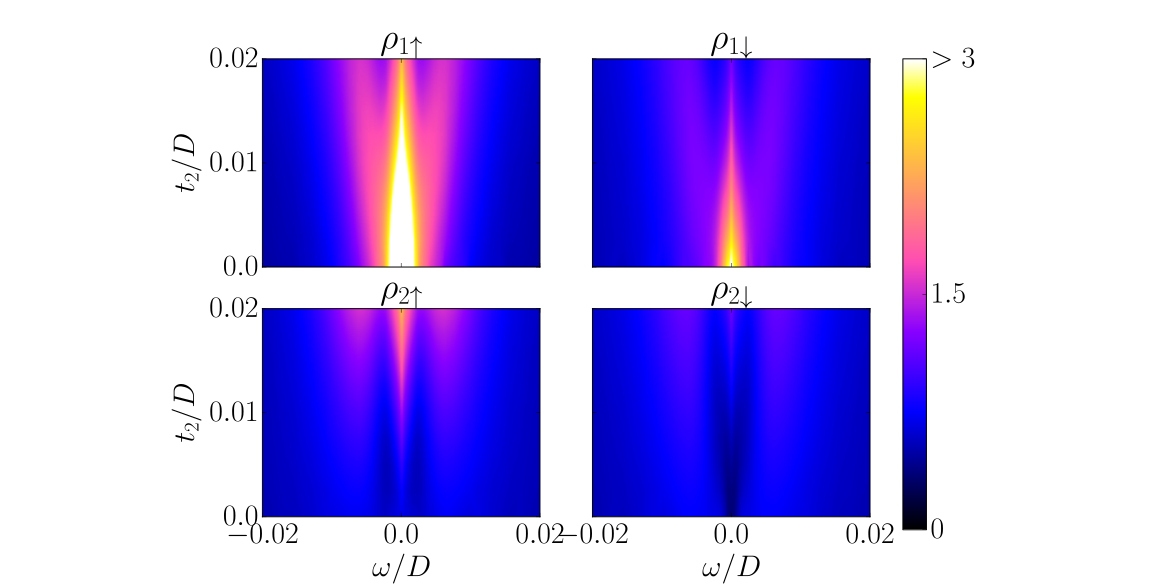
\includegraphics[scale=0.35]{IMAGES/ed2/2D.png}
% \caption{\label{fig:2D/Shift_ed2} Evolution of the DOS of both QDs through the $\ed{2}$ tuning. UP: QD1. DOWN: QD2. LEFT: Spin $\up$. RIGHT: Spin $\dw$.}
% \end{figure}



% -------------------FIGURES EVOLUTION ED--------------------


%-----------E N D  F I G U R E  4 ------
\begin{figure}[bt]
    \begin{center}
    \includegraphics[scale=0.41]{IMAGES/NRG/t2>0.png}
    \caption{  \label{fig:Nt2>0} The same as in \ref{fig:t1=t2} for the  interacting DOS for interacting dots coupled in series (\ref{fig:MajoranaModels}(c)). Inset in b): Zoom to low-energy DOS. \protect\Source{}
    }
    %
    \end{center}
    \end{figure}



    Finally, \ref{fig:Nt2>0} shows the NRG results for the last configuration, where the dots are coupled in series \ref{fig:MajoranaModels}(c). Notably, the indirectly-attached MZM exhibits a robust type II Majorana signature in the first dot over a destroyed Kondo peak. This is observed clearly in  \ref{fig:logc} where $\rho_{1\dw}$ exhibits a constant $\frac{0.5}{\pi \Gamma_1}$-height Majorana peak  . This signature is stable under the gate voltage tuning in dot $1$ and similar results are obtained in dot $2$ . In addition, only  in the particle hole symmetric case the second dot presents a type II Majorana signature (Inset \ref{fig:Nt2>0}(b)). 

    We could understand this effect by thinking that the dots in model (c) are attached in series. Therefore both QDs can be thought as extensions of the Kitaev chain, were the first dot is the last place in the wire. Hence the Majorana should be localized at this dot despite the application of gate voltages. This situation is similar to the case of a single dot attached to a Majorana chain, where it is known that the MZM appears in the dot even when this is supposed to be empty \cite{vernek_subtle_2014}. It still remains the doubt about why this effect is not observed in the non-interacting case . On the other hand, there is a Fano resonance at the Fermi energy in the spin-$\dw$ DOS  \ref{fig:Nt2>0}(d)(e) . This zero mode was not identified as a potential Majorana signature since it varies with the values of $\Delta \ep_1$ (\ref{fig:logc}) and $\Delta \ep_2$.
    

We are now writing a paper summarizing these results. As we observed, we were able to characterize the transitions of the Majorana signature in different geometric arrangements of the dots. In the following section we will present some ideas that are still in development. We hope they could lead us to future publications

\section{Additional  results}

\begin{figure}[t]
\centering
\includegraphics[scale=0.45]{IMAGES/NRG/Indirect.png}
\caption{\label{fig:indirect} Dependence of the DOS in the symmetric model \ref{fig:MajoranaModels}(a) over $t_1=t_2$ and $\omega$. Up: High energy . Down: Zoom to low energy states.  \protect\Source{}}
\end{figure}

This section contains additional results which we are considering to study in  future publications. 

\subsection{Indirect exchange through the Majorana mode}

In \ref{fig:NRG_Majorana} we observed the emergence of satellite peaks at low energies product of anti-ferromagnetic exchange interactions. This exchange interaction can occur through the lead and through the Majorana mode. The reason why we are observing just two satellites is because the Majorana  couplings $(t_1=t_2)$ and the broadening parameters $(\Gamma_1 = \Gamma_2)$ are about the same order. Hence the peaks are a superposition of both exchange interactions. 

We can separate both exchange interactions by observing the dependence of the DOS at different orders of $t_1=t_2$ in \ref{fig:indirect}. We can distinguish two regimes:

\begin{figure}[t]
\centering
\includegraphics[scale=0.5]{IMAGES/NRG/Lowt1=t2.png}
\caption{ \label{fig:indirectLow} Dependence of the DOS in the symmetric model \ref{fig:MajoranaModels}(a) over $t_1=t_2$ and $\omega$. Up: High energy . Down: Zoom to low energy states.  \protect\Source{}}
\end{figure}

\begin{enumerate}
 \item Low Majorana coupling $t_1=t_2 < 0.5$: Two additional satellite peaks appear in the spin-$\dw$ DOS (See inset in \ref{fig:indirectLow} for better appreciation). These peaks are similar to the  Kondo satellites that appear at high energies. However, since they appear only at low-energies, it is clear that they are produced by the MZM. We conclude that these two satellites are produced by the indirect exchange through the attached  Majorana quasi-particle. 
 \item High Majorana coupling $t_1=t_2 > 0.5$: When the Majorana coupling is high enough, the indirect exchange through the MZM occurs in the same energy scale as the Kondo satellites. Notably, the spin-$\dw$ satellite peaks in the high energy regime are not affected by this effect. Instead, a visible inflation of the satellites in the spin-$\up$ DOS is observed. Therefore the MZM is actually correlated with the spin-$\up$ DOS through the satellite peaks. This is unexpected since the Majorana is only coupled to the spin-$\dw$ channel.  The only explanation for this is that these satellites are formed by a strongly correlated state between the MZM, the dot states and the lead. 
\end{enumerate}
\begin{figure}[h]
\centering
\includegraphics[scale=0.64]{IMAGES/NRG/IND.png}
\caption{\label{fig:IND} DOS at both dots for the model in the left inset. The right inset zooms the low-energy DOS in the second dot.\protect\Source{} }
\end{figure} 

% \begin{figure}[t]
% \centering
% \includegraphics[scale=0.6]{IMAGES/NRG/Indirect.png}
% \caption{\label{fig:indirectLow} Dependence of the DOS in the symmetric model \ref{fig:MajoranaModels}(a) over $\omega$ for $t_1=t_2 = 0.1\Gamma_1$ (Low energy regime). Left inset: Majorana model. Right inset:Low energy regime. Majorana exchange peaks can be observed.  \protect\Source{}}
% \end{figure}



\subsection{Indirect Majorana coupling through the lead}

Imagine a model were we connect both dots symmetrically to the leads but we only connect the MZM to the first dot. In addition, we do not allow inter-dot tunneling. Then the only connection between the MZM and the second dot would be passing through the first dot and  the lead. We didn't expect to see any Majorana signature in the second dot in these conditions. However, \ref{fig:IND} shows a clear type I Majorana signature in the second dot.




 Note also that the density of states in the second dot is very small in comparison with the first dot. This is intriguing since this dot is directly connected with the lead and it is still at the Kondo regime. This ambiguity means that the zero-bias DOS is favored by a direct coupling to an MZM.  

\subsection{Critical behavior in  zero-bias DOS }

In \ref{fig:Nt1>0}(f) we observe a sharp peak at DOS. This peak is actually a big problem for our results since they are  supported on the spectral densities at the Fermi energy. In \ref{fig:Critical} we observe a critical behavior in the zero-bias DOS close to $\Delta\epsilon_2 =0$. This is quite intriguing . 


\begin{figure}[t]
\centering
\includegraphics[scale=0.5]{IMAGES/NRG/Critical.png}
\caption{\label{fig:Critical} Logarithmic dependence of the DOS in the second dot for setup in \ref{fig:MajoranaModels}(b) over the second gate voltage. Cut at $5\Gamma_1$ corresponds to \ref{fig:Nt1>0}(f). \protect\Source{} }
\end{figure} 
 States (DOS). The method used to compute the DOS is the Density Matrix numerical renormalization Group (DM-NRG). A complete description of this algorithm will be given in the following sections.  \\

% For now, we proceed to describe how the NRG is applied to solve the Anderson model in a QD:\\

% \Jesus{I still need to do a long revision to this section. Probably I will send most of the computations to the abstract and leave a summary of NRG and its advantages in the main text.}







%\begin{figure}[h]
%\centering
%\includegraphics[scale=0.5]{IMAGES/NRGchain.png}\caption{\label{FigNRG-chain} Chain-Hamiltonian describing the Anderson model.
%The chain starts at the initial dot hamiltonian $H_{d}$. The $f_{m}^{\dagger}$'s
%are the creation operators at the $n^{\mbox{th}}$-site of the chain.
%The $\xi_{n}$'s describe the magnitude of the interaction between
%consecutive sites. }
%\end{figure}




\subsection{Iterative diagonalization in a single QD attached to a metallic lead \label{subsec:QD-Diag} }

Now that we have an iterative representation of the Anderson Model
Hamiltonian \eqref{eq:Newchain-Hamiltonian}, we will describe how the NRG code works for a QD attached to a lead. We start with the dot Hamiltonian.

\begin{equation}
H_{d}=\frac{1}{D}\left(\epsilon+\frac{U}{2}\right)d_{\sigma}^{\dagger}d_{\sigma}+\frac{U}{2D}(d_{\sigma}^{\dagger}d_{\sigma}-1)^{2}.\label{eq:DotHam}
\end{equation}


\noindent Now observe that Hamiltonian \eqref{eq:DotHam} is already in the
diagonal form for the basis $\left\{ \vert\uparrow\!\downarrow\rangle,\vert\uparrow\rangle,\vert\downarrow\rangle,\vert0\rangle\right\} $
\[
H_{d}=\frac{1}{D}\left[\begin{array}{cccc}
2\epsilon+\frac{3U}{2} & 0 & 0 & 0\\
0 & \epsilon+\frac{U}{2} & 0 & 0\\
0 & 0 & \epsilon+\frac{U}{2} & 0\\
0 & 0 & 0 & \frac{U}{2}
\end{array}\right].
\]


Lets define $H_{-1} := \frac{2 H_d \Lambda^{-1/2}}{1+\Lambda^{-1}}$ as in \ref{eq:H-1}. It is convenient here to define unit-less variables $\epsilon' =\frac{2\epsilon \Lambda^{-1/2}}{D(1+\Lambda^{-1})}, U'= \frac{2U\Lambda^{-1/2}}{D(1+\Lambda^{-1})}$ and $\Gamma':=\sqrt{\frac{2\Gamma}{\pi D}}$. Then adding the first site of the Wilson's chain interaction to $H_{d}$ we obtain a new Hamiltonian of the form 

\begin{equation}
H_{0}=\Lambda^{\frac{1}{2}}H_{-1}+\Gamma'\left(d_{\sigma}^{\dagger}f_{0\sigma}+f_{0\sigma}^{\dagger}d_{\sigma}\right).\label{eq:H0fromH-1}
\end{equation}



The Hilbert space for this mew Hamiltonian must be extended to include
the $4$ degrees of freedom of the $f_{0\sigma}^{\dagger}$ particles,
which are given by $\left\{ \vert\uparrow\!\downarrow\rangle,\vert\uparrow\rangle,\vert\downarrow\rangle,\vert0\rangle\right\} $.
Therefore, the total Hilbert space for $H_{0}$ is given by a base
of the form 
\[
\vert s_{1}\rangle\vert s_{2}\rangle:=\vert s_{1}\rangle\otimes\vert s_{2}\rangle\mbox{ with }\vert s_{i}\rangle\in\left\{ \vert\uparrow\!\downarrow\rangle,\vert\uparrow\rangle,\vert\downarrow\rangle,\vert0\rangle\right\} .
\]


\noindent We obtain an space of dimension $4\times4=16.$ Now, before adventuring
to write the Hamiltonian for $H_{0}$ as a $16\times16$-matrix note
that $H_{-1}$ preserves the total particle number $\mathcal{N}$ and the total spin $S$. We can associate each state to one of these symmetries as 

\begin{align}
\vert \uparrow\downarrow\rangle\longrightarrow\vert \mathcal{N}=2,S=0\rangle\ ,& \ \vert0\rangle\longrightarrow\vert \mathcal{N}=0,S=0\rangle \\ 
\vert \uparrow\rangle\longrightarrow\vert \mathcal{N}=1,S=\frac{1}{2}\rangle\ ,& \ \vert \downarrow \rangle\longrightarrow\vert \mathcal{N}=1,S=\frac{-1}{2}\rangle.
\end{align}

The propagation rule for the symmetry is defined with the following identity 
\begin{equation}
  \vert \mathcal{N}_{1},S_{1}\rangle\otimes\vert \mathcal{N}_{2},S_{2}\rangle\subset\vert \mathcal{N}_{1}+\mathcal{N}_{2},S_{1}+S_{2}\rangle \label{eq:PropRuleQD}
\end{equation} 
  

 \noindent Then we can use  $\mathcal{N}$ and $S$ as quantum numbers to generate the the block structure of $H_{0}$ . We will observe that the terms in the diagonal will correspond to the eigenvalues of $H_{-1}$ for the first space. The non-diagonal terms are the result of the hopping interactions with the first site. 

\begin{multicols}{2}

$H_{\mathcal{N}=0,S=0}:$
\[
\begin{array}{c}
\vert0\rangle\vert0\rangle\rightarrow\end{array}\begin{array}{c}
\left[\frac{U'}{2}\right]\end{array}
\]


$H_{\mathcal{N}=4,S=0}:$
\[
\begin{array}{c}
\vert\uparrow\!\downarrow\rangle\vert\uparrow\!\downarrow\rangle\rightarrow\end{array}\begin{array}{c}
\left[2\epsilon'+\frac{3U'}{2}\right]\end{array}
\]


\end{multicols}

\begin{multicols}{2}

$H_{\mathcal{N}=1,S=\frac{1}{2}}:$
\[
\begin{array}{c}
\vert\uparrow\rangle\vert0\rangle\rightarrow\\
\vert0\rangle\vert\uparrow\rangle\rightarrow
\end{array}\left[\begin{array}{cc}
\epsilon'+\frac{U'}{2} & \Gamma'\\
\Gamma' & \frac{U'}{2}
\end{array}\right]
\]


$H_{\mathcal{N}=1,S=\frac{-1}{2}}:$
\[
\begin{array}{c}
\vert\downarrow\rangle\vert0\rangle\rightarrow\\
\vert0\rangle\vert\downarrow\rangle\rightarrow
\end{array}\left[\begin{array}{cc}
\epsilon'+\frac{U'}{2} & \Gamma'\\
\Gamma' & \frac{U'}{2}
\end{array}\right]
\]


\end{multicols}

\begin{multicols}{2}

$H_{\mathcal{N}=2,S=-1}:$
\[
\begin{array}{c}
\vert\downarrow\rangle\vert\downarrow\rangle\rightarrow\end{array}\begin{array}{c}
\left[\epsilon'+\frac{U'}{2}\right]\end{array}
\]


$H_{\mathcal{N}=2,S=1}:$
\[
\begin{array}{c}
\vert\uparrow\rangle\vert\uparrow\rangle\rightarrow\end{array}\begin{array}{c}
\left[\epsilon'+\frac{U'}{2}\right]\end{array}
\]


\end{multicols}


$H_{\mathcal{N}=2,S=0}:$
\[
\begin{array}{c}
\vert\uparrow\!\downarrow\rangle\vert0\rangle\rightarrow\\
\vert\uparrow\rangle\vert\downarrow\rangle\rightarrow\\
\vert\downarrow\rangle\vert\uparrow\rangle\rightarrow\\
\vert0\rangle\vert\uparrow\!\downarrow\rangle\rightarrow
\end{array}\left[\begin{array}{cccc}
2\epsilon'+\frac{3U'}{2} & \Gamma' & -\Gamma' & 0\\
\Gamma' & \epsilon'+\frac{U'}{2} & 0 & \Gamma'\\
-\Gamma' & 0 & \epsilon'+\frac{U'}{2} & -\Gamma'\\
0 & \Gamma' & -\Gamma' & \frac{U'}{2}
\end{array}\right]
\]


\begin{multicols}{2}

$H_{\mathcal{N}=3,S=\frac{1}{2}}:$
\[
\begin{array}{c}
\vert\uparrow\!\downarrow\rangle\vert\uparrow\rangle\rightarrow\\
\vert\uparrow\rangle\vert\uparrow\!\downarrow\rangle\rightarrow
\end{array}\left[\begin{array}{cc}
\epsilon'+\frac{U'}{2} & -\Gamma'\\
-\Gamma' & \frac{U'}{2}
\end{array}\right]
\]


$H_{\mathcal{N}=3,S=\frac{-1}{2}}:$
\[
\begin{array}{c}
\vert\uparrow\!\downarrow\rangle\vert\downarrow\rangle\rightarrow\\
\vert\downarrow\rangle\vert\uparrow\!\downarrow\rangle\rightarrow
\end{array}\left[\begin{array}{cc}
\epsilon'+\frac{U'}{2} & -\Gamma'\\
-\Gamma' & \frac{U'}{2}
\end{array}\right]
\]


\end{multicols}

\begin{figure}[t]
	\subfloat[$N$ takes only even values]{\includegraphics[scale=0.5]{IMAGES/even.png}}\subfloat[$N$ run only through odd values]{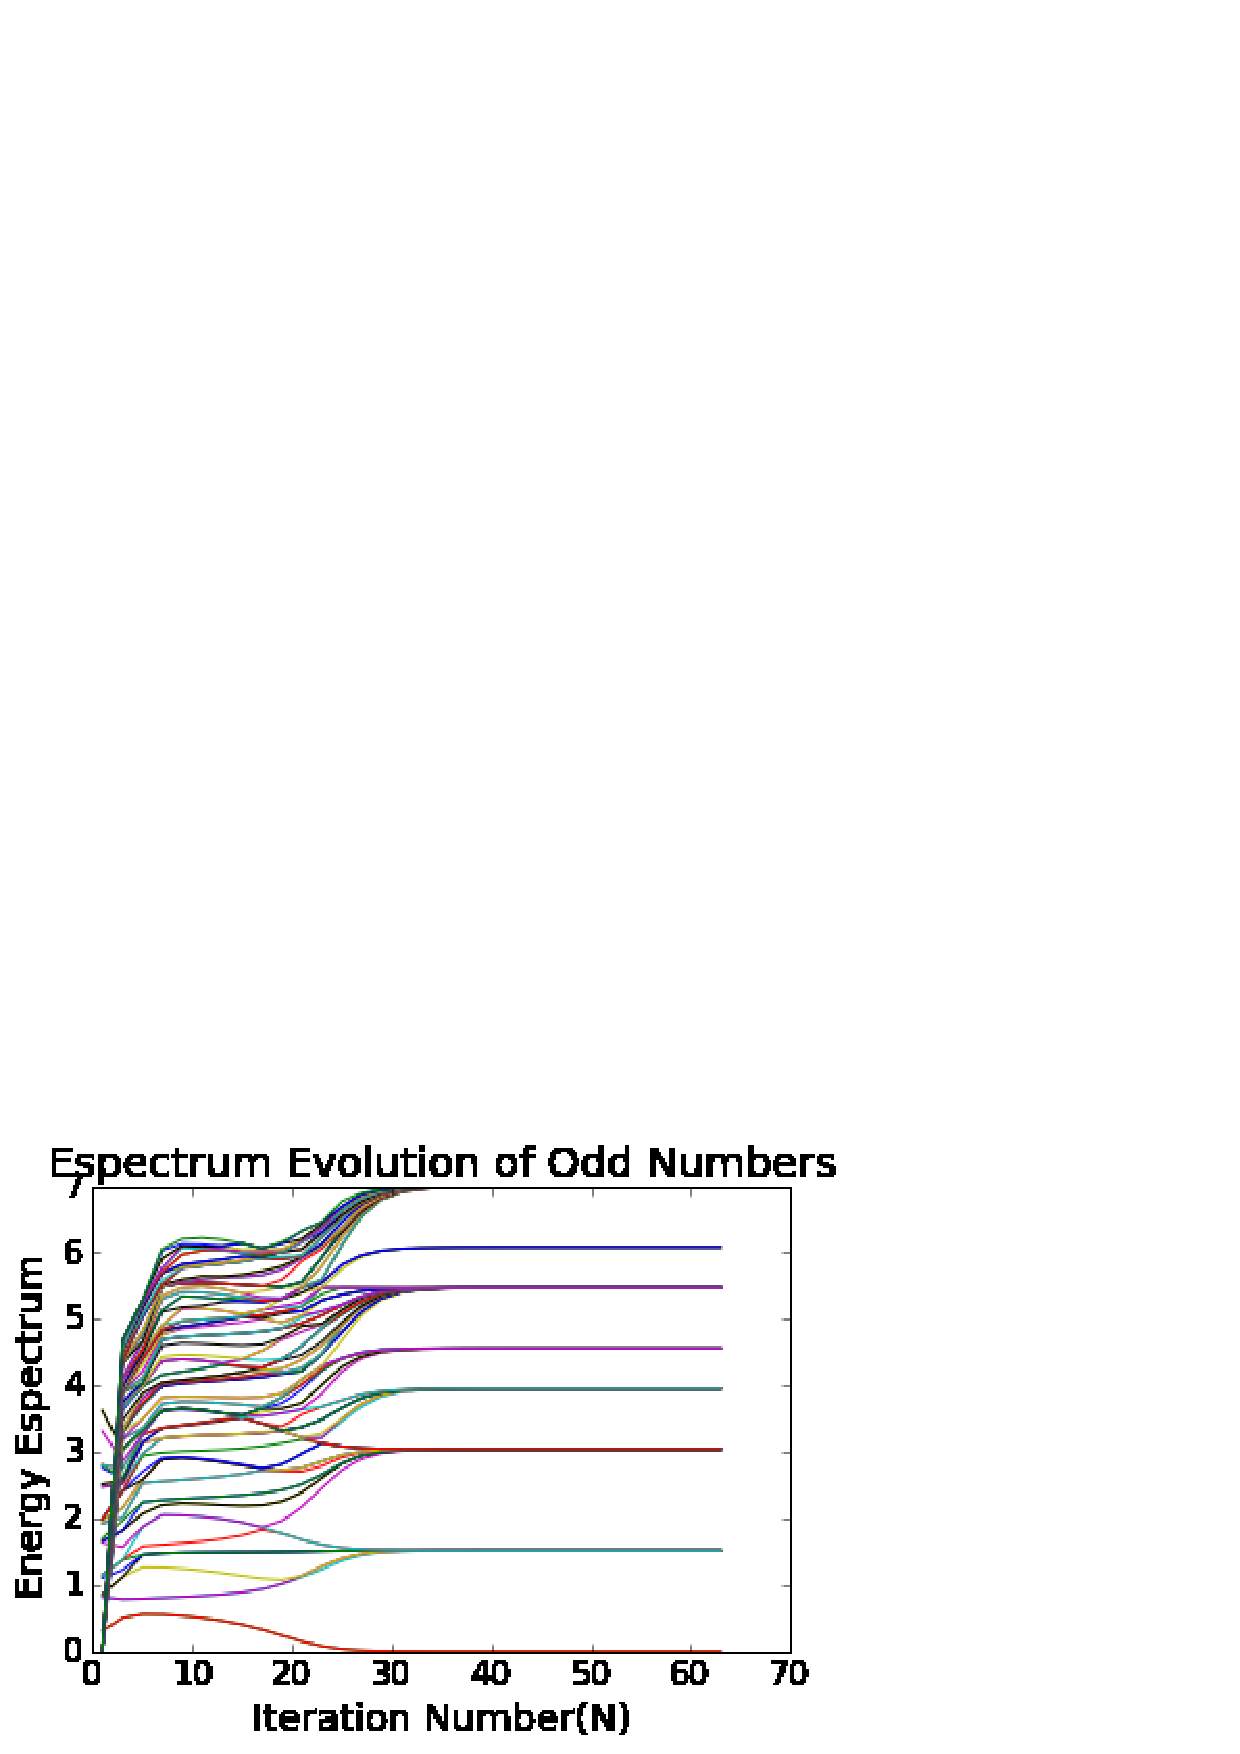
\includegraphics[scale=0.5]{IMAGES/odd.png}}\caption{\label{Fig-Dot-Spectrum} Evolution of the QD-spectrum vs number of
	iterations of the code for $U'=0.5,\ \ep'=-0.25,\ \Gamma=2.82\times10^{-2}.$ }
\end{figure}

The next step would be to diagonalize $H_{0}$ by blocks $(H_{\mathcal{N},S})$ and then including the next place in the chain. The following Hamiltonians are generated in the same way from equation \eqref{eq:NRG-Renormalization}. The symmetries of the new states can be obtained from the propagation rule \eqref{eq:PropRuleQD}. When the number of states surpasses the 1000 states, the code will automatically cutoff the higher energy states. However it is important that a Block is not divided in this cutting, since it could break the preserved symmetry. 

Finally, the spectrum for $\Lambda = 2.5$ takes the 'spaghetti' form in \ref{Fig-Dot-Spectrum}.  Note that before $N=30$, the low-energy contributions generate significant changes in the energy levels.  However, the stable spectrum after the step $N=30$ is a signature that the code has converged. As we previously declared, it is not $\mathcal{T}$ but $\mathcal{T}^2$ the transformation that has fixed points, which explains why it was necessary to plot the even and the odd spectrum separately.

% The resulting eigenvectors will be characterized by both quantum numbers
% so that we can write them in the form $\vert N,S,i\rangle$ with $i$
% taking as many values as the degeneracy of its block. For higher values of $N$,

% We now proceed by induction supposing that for each $N$ the Hamiltonian $H_{N}$ is already diagonalized and the eigenvectors are organized in states with labels $\vert N,S,i\rangle.$ The next step will be to add the $4$-Hilbert space corresponding to $f_{N+1,\sigma}$ organized the eigenvectors according to the quantum numbers $\vert N',S',i\rangle$ and proceed to diagonalize by blocks the new Hamiltonian. Apart of it, the code must have a cutoff to the number of states. \\

At the end of the NRG code, we obtain a complete list of the spectrum $(E_{i, N})$ and the eigenstates $(\vert i , N \rangle)$ of the Hamiltonian at each step $N$ of the chain ( See \ref{Fig-Dot-Spectrum}). It is important to keep all of these states since each one of them represents different thermodynamic regimes of the system. While the site $N=1$ represents the physics of the system relevant at temperatures around $\frac{D \Lambda^{-1}}{K_B }$, the site $N=30$ shows the low energy contributions at $T \sim \frac{D \Lambda^{-30}}{K_B }$ where the ground state is strongly correlated. Furthermore, the states at low temperatures are entangled with the higher energy states. We need to take this into account to extract dynamical quantities of the system, which is the objective of the following section. 

\subsection{The Density Matrix Renormalization Group (DM-NRG) \label{subsec:DM-NRG}}
The NRG codes allows us to compute several thermodynamic quantities such as the entropy $S$, the free energy and the partition function $Z(\beta)$. In addition, we can compute the spin magnetization or dynamical quantities such  the density of states, the magnetic susceptibility and the conductivity. To perform this we can use the spectrum obtained in the NRG code to define the Boltzman distribution of the system. Then we apply the usual methods of statistical mechanics.  

% It is necessary to embed NRG with the faculty to compute these operators at each step $N$ of the code. {} 

In this thesis we will focus in computing the density of states at the impurity (QD). For this, let $\vert j\rangle$ and $\vert q \rangle$ label a base of eigenstates of the Hamiltonian $H$. Now recall the definition of the retarded green function \eqref{eq:TempGreen}

\begin{align}
G_{d,d^{\dagger}}(t)&=\theta(t)\left\langle \{ d(t)d^{\dagger}(0) \} \right\rangle \\ \label{eq:MeanGreen}
&=\theta(t)\left\langle \left[e^{\frac{i}{\hbar}Ht}de^{-\frac{i}{\hbar}Ht}d^{\dagger}\right]\right\rangle +\theta(-t)\left\langle \left[d^{\dagger}e^{\frac{i}{\hbar}Ht}de^{\frac{-i}{\hbar}Ht}\right]\right\rangle \\
&=\theta(t)\sum_{\vert j\rangle,\vert q\rangle}p_{j}\langle j\vert e^{\frac{i}{\hbar}Ht}d\vert q\rangle\langle q\vert e^{-\frac{i}{\hbar}Ht}d^{\dagger}\vert j\rangle+\theta(-t)\sum_{\vert j\rangle,\vert q\rangle}p_{q}\langle q\vert d^{\dagger}e^{\frac{i}{\hbar}Ht}\vert j\rangle\langle j\vert de^{-\frac{i}{\hbar}Ht}\vert q\rangle\\
&=\theta(t)\sum_{\vert j\rangle,\vert q\rangle}p_{j}e^{\frac{-i}{\hbar}t\left(E_{j}-E_{q}\right)}\left\Vert \langle j\vert d\vert q\rangle\right\Vert ^{2}+\theta(-t)\sum_{\vert j\rangle,\vert q\rangle}p_{q}e^{\frac{i}{\hbar}t\left(E_{j}-E_{q}\right)}\left\Vert \langle j\vert d\vert q\rangle\right\Vert ^{2}
\end{align}

\noindent Where $p_{j}:=\frac{e^{-\beta E_{j}}}{Z(\beta)}$ defines the Boltzmann probability of the eigenstate $\vert j\rangle$ according to Hamiltonian $H$. 

It is known that the Fourier transform of an expression of the form ${\displaystyle e^{-ax}\theta(x)}$ is $\frac{1}{\omega+is-a}$. Then the Green function in the energy domain is 
\begin{equation}
\Green{d,d^{\dagger}}=\frac{1}{Z(\beta)}\sum_{\vert j\rangle,\vert q\rangle}{\displaystyle \frac{e^{-\beta E_{j}}+e^{-\beta E_{q}}}{\omega+is-E_{j}+E_{q}}}\left\Vert \langle j\vert d\vert q\rangle\right\Vert ^{2}
. \label{eq:greenT}
\end{equation}

\noindent From the imaginary part of \eqref{eq:greenT} we obtain a formula for the spectral density in terms of the eigenstates and energies of the Hamiltonian 
\begin{equation}
\rho_{d}=\frac{1}{Z(\beta)}\sum_{\vert j\rangle,\vert q\rangle}{\displaystyle \left(e^{-\beta E_{j}}+e^{-\beta E_{q}} \right) \delta\left(\omega-E_{j}+E_{q} \right) } \left\Vert \langle j\vert d\vert q\rangle \right\Vert^{2}. \label{eq:DOSeigenstates}
\end{equation}

\noindent This new expression for the DOS can be integrated into  the NRG code in different ways . A first method created by Costi \textit{et al.} consists in computing \eqref{eq:DOSeigenstates} with the eigenstates of each shell Hamiltonian $H_N$  \cite{costi_transport_1994}. It is necessary to take into account that the operator $ d$ is constantly rotating after each diagonalization procedure, which produces different representations at each shell Hamiltonian basis. Then, an important part of Costi's algorithm is to obtain these new representations of $d$ at the $H_N$-basis $(\langle j\vert d\vert q\rangle\Vert_N)$ recursively starting from an input representation $\langle j\vert d\vert q\rangle\Vert_{N=0}$.

Although Costi's method predicts accurately the DOS at low-energies, it fails to fit the high energy levels. The method that corrects this problem receives the name of Density Matrix Numerical Renormalization Group (DMNRG) \cite{hofstetter_generalized_2000}. The main idea of DMNRG is to include the entanglement corrections with the lower energy-states using the density matrix formalism. For this, Hofstetter defines the density matrix at the last shell Hamiltonian $N_{max}$ $\hat{\rho}$ as the thermal mixed state 

\begin{equation}
\hat{\rho}_{N_{max}} = \sum_{j}e^{-\beta E_{j}}\vert j          \rangle_{N_{max}} \langle j\vert, \label{eq:rho_n}
\end{equation}

\noindent where the subindex $N_{max}$ suggests that $\vert j \rangle_{N_{max}} \langle j\vert$ is an eigenstate of the last shell Hamiltonian $H_{N_{max}}$. 

With this new density matrix, we could rewrite \eqref{eq:MeanGreen} as 
\begin{equation}
G_{d,d^{\dagger}}^{N_{max}}(t) = \text{Tr} \left( \hat{\rho}_{N_{max}}\theta(t)\left\{ d^{\dagger}(t),d(0)\right\} \right). 
\end{equation}
\noindent From the Green function $G_{d,d^{\dagger}}^{N_{max}}(t)$ we can obtain the density of states associated to the temperature $T_{N_{max}}$. Nevertheless, these results are not relevant at higher temperatures. 

\begin{figure}
\centering
\includegraphics[scale=1]{IMAGES/DQD/DMRGchain.png}
\caption{\label{fig:OpenQuantum} Wilson's chain depicted as an open quantum system. Adapted from \cite{hofstetter_generalized_2000}.  }
\end{figure}

To solve this problem we may think Wilson's chain as an open quantum system where the environment are the low-energy sites of the chain and the system $(\rho_{red})$ contains the high-energy sites including the QD-impurity  as observed in \ref{fig:OpenQuantum}. Using this analogy,  we can readily obtain the density matrix $\rho_S$ by taking the partial trace over the environment

\begin{equation}
\rho_{sys} = \text{Tr}_{env}[\rho_{N_{max}}].
\end{equation} 

The DM-NRG code applies recursively this idea to obtain the density matrix corresponding to each scale of temperature $T_N$. It starts from $\rho_{N_{max}}$ defined at \eqref{eq:rho_n} and obtains $\rho_{N_{max}-1} $ by taking the partial trace over the vector space corresponding to the last site of the chain
\begin{equation}
\rho_{N_{max}-1} = \text{Tr}_{N_{max}}[\rho_{N_{max}}].
\end{equation}
\noindent The other density matrices are computed by induction as 
\begin{equation}
\rho_{N-1} = \text{Tr}_{N}[\rho_{N}],
\end{equation}
and the density of states at each temperature regime can be computed from the green function 
\begin{equation}
G_{d,d^{\dagger}}^{N} (t) = \text{Tr} \left( \hat{\rho}_{N}\theta(t)\left\{ d^{\dagger}(t),d(0)\right\} \right). 
\end{equation}

The DM-NRG algorithm produces significantly better results  at high energies than Costi's initial idea. Indeed, DM-NRG is still one of the best methods to compute dynamic quantities of an impurity system. In the following subsection we will give some details of how DM-NRG is integrated with the NRG code. 


% Then, we could rewrite equation  \eqref{eq:MeanGreen} as 
% \begin{equation}
% G_{d,d^{\dagger}}(t)\left = \text{Tr}\left(\hat{\rho}_{N}\mathbb{T}\left[\left\{ d^{\dagger},d\right\} \right]\right). 
% \end{equation}
% But this result will only give us the result 


% But the density matrix $\hat{\rho}_{N}$ is different from \hat{\rho}_{N}$. In other 



% In this formalism the expression at

% However this last method neglected the strong correlation between the low and high energy states in the systems. 



% To compute  dynamical quantities  like the density of states we used the density matrix renormalization group approach . 



\subsection{Specifications of the NRG Code }

The NRG code used in this thesis was implemented by my thesis advisor Luis Gregorio Dias during his posdoc at the University of Ohio.  The general scheme  is shown in \ref{fig:Code}. It incorporates different stages.. Here we give a brief description of them:

\begin{figure}[t]
\centering
\includegraphics[scale=0.4]{IMAGES/NRG/NRGcode.png}
\caption{\label{fig:Code} Diagram of the NRG code}
\end{figure}

\begin{itemize}
\item \textbf{Model:} The model defines the type of impurity that we are going to study. It could be a single QD or more complex structures such as a DQD or a Majorana-QD system. My main contribution to this code was at this stage. I designed the mode DQD-Majorana, which describes a DQD coupled to a Majorana zero mode. These models preserve different symmetries. In the single dot Hamiltonian presented in \ref{subsec:QD-Diag} we used the symmetry $\mathcal{N}S_z$, which is equivalent to charge-spin $QS_z$. However we will find that Majorana systems  require another  symmetry-type that we call as $N\up P\dw$. The model is defined by an initial Hamiltonian $H_{-1}$ and the annihilation operators $d_{i\sigma}$ which must be submitted in the code written in the block symmetry representation described in \ref{subsec:Syms}.
\item \textbf{Input:} The input is a '.dat'-file that attributes a numerical value to each parameter of the model. In addition, it allows to set different code specifications as the number of iterations $N_{max}$, the scaling parameter $\Lambda$ and the maximum number of states before the cut-off. It is also possible to include additional implementations to improve the results of the NRG code such as the Z-trick \cite{oliveira_generalized_1994} and the Complete Fock State. In this project, we only used the Z-trick, which significantly improves the spectral resolution at high energies.
\item \textbf{NRG:} This part of the code mainly integrates the ideas of \ref{subsec:Logarithmic} and implements the iterative diagonalization described in \ref{subsec:IterativeDiag}. Each shell Hamiltonian $H_n$ is diagonalized. The high-energy eigenstates are cut-off if they exceed the maximum limit. Then, the states are rotated and the eigenvalues are rescaled to include the next step of the Wilson's chain. The symmetry block structure is preserved during the entire loop. NRG's output is a detailed evolution of the spectrum which produces the spaghetti form. In addition, it can print the states and operators that are necessary to start other instances of the code like DM-NRG.
\item \textbf{Site $N+1$:} This is an small class that creates another site of the chain in the base $\left\{ \vert\uparrow\!\downarrow\rangle,\vert\uparrow\rangle,\vert\downarrow\rangle,\vert0\rangle\right\} $ . This base must be rewritten according to the symmetry quantum number. It is coupled with the matrices at the NRG code. 
\item \textbf{DM-NRG}: As described in \ref{subsec:DM-NRG}, this code generates iteratively the density matrix associated to each energy scale . Then it computes the green function and the density of states. The DOS of the single QD model is an example of its outputs. The plot shows the characteristic Kondo peak at the Fermi energy in the middle of the Coulomb peaks describing the energy states. 
\end{itemize}

 This NRG code is implemented in C++. It can be cloned from the Github link \url{https://git.io/fh9cM}.  To optimize the performance of NRG, the code uses the packages Boost, LAPACK and Gnu Scientific Library (GSL), which provide a rapid interface for numerical matrix diagonalization. 
 




  % language by the advisor of this thesis. In \ref{Fig-Dot-Spectrum} we observe the evolution of the spectrum of the Hamiltonian according to the number of iterations of the code. As we can appreciate, this evolution converges for even and odd number around $N=30$.  \\{}





\subsection{NRG results in a double quantum dot coupled to a metallic lead\label{sec: NRG-DQD}}

\begin{figure}[bt]
     \centering
    \subfloat[ Single QD-lead system \label{fig:NRG-1D}]{\includegraphics[scale=0.6]{IMAGES/DQD/NRG-QD.png}}
     \subfloat[Symmetric coupling \label{fig:NRGDQD-G2}]{\includegraphics[scale=0.45]{IMAGES/DQD/NRG-DQD.png}} \\
    \subfloat[\label{fig:NRGDQD-tdots} T-junction of the dots. Low energy DOS. ]{\includegraphics[scale=0.5]{IMAGES/DQD/NRG-IndirectDQD.png}}
    
     \caption{\label{fig:NRG-DQD} Density of states for the DQD attached to the lead at different configurations. Left insets: Setup that is being used. Right insets: Low energy DOS.  \protect\Source{ }}
\end{figure}


We now intend to observe the results of this code applied to the model double quantum dot attached to a metallic lead. The  Hamiltonian for this system is the Anderson model with the impurity described by the interacting version of Hamilonian \eqref{eq:HDQD}

\begin{equation}
H_{DQD}=\sum_{i=1}^2\sum_\sigma \left( \epsilon_{i} + \frac{U_i}{2} \right) d_{i\sigma}^{\dagger}d_{i\sigma} + \left(\sum_{i\sigma} d_{i\sigma}^{\dagger}d_{i\sigma} -1 \right)^2 + \sum_\sigma t_{dots}d_{1\sigma}^{\dagger}d_{2\sigma}+t_{dots}^*d_{2\sigma}^{\dagger}d_{1\sigma}
\label{eq:interactingDQD}
\end{equation}

\noindent The Hilbert space of this system has $16$-dimensions and the symmetries in this Hamiltonian are exactly the same than the ones in the single QD case $\mathcal{N}S$. Nevertheless, we decided to test the DQD-Majorana mode in this system. By setting the Majorana couplings to $t_1=t_2= 0$ we can decouple the Majorana mode, hence obtaining the DQD model (See \ref{chap:Results}). The results we obtained are in agreement with previous previous papers \cite{dias_da_silva_transmission_2008}, which was an important test to confirm the veracity of this new mode. 

For the entire thesis we will fix the value of the coulomb repulsion parameters to 
\begin{equation}
 U_1 = U_2 = 17.7305 \Gamma_1.
\end{equation}
\noindent We picked these parameters considerably higher than the broadening unit $\Gamma_1$ to guarantee the appearance of Kondo physics at visible temperatures in comparison with the Coulomb peak.  

%Still need to correct this ... but for know.... PAPER!



 NRG-code  We used the same configurations from \ref{fig:GreenDQD}. The  results appear in \ref{fig:NRG-DQD}:

 \begin{enumerate}
 
\item The single QD attached to a metallic lead is a particular case of the double quantum dot model, where the second dot is not attached $\Gamma_2 = t_{dots}=0$.  \ref{fig:NRG-DQD} shows the NRG results for this case. The three plots show the external Coulomb peaks at $e_1 = \frac{U}{2} \sim 8.62\Gamma_1$, which represent the DOS of the energy levels. In addition  Figure \ref{fig:NRG-1D} shows a central peak at the Fermi energy. Note, that there shouldn't be a state in this position since it is inside a gap between two energy levels (Coulomb peaks).\textbf{This is the Kondo Peak} \cite{hewson_kondo_1997}. This peak explains the zero-bias platoes in \ref{fig:ExpKondo}.  
\item 
In Figure \ref{fig:NRGDQD-G2} we observe the DOS when the two QDs are symmetrically attached.  At low energies, the inset shows the appearance of two satellite peaks representing the Ruderman-Kittel-Kasuya-Yosida (RKKY) interaction. This is an anti-ferromagnetic coupling that appears in the interacting case due to the strong correlations between both dots. 

% A detailed explanation  these new states is included in \ref{sec:DoublePeak}.  
\item The most interesting case is in Figure \ref{fig:NRGDQD-tdots}. As we already observed in the non-interacting case, the interference with the second dot completely destroys the zero mode which is now formed by the Kondo peak. This effect is observed at low energies closed to $t_{dots}=0.689\Gamma$. The paper describing this result was a central part of one of my advisor's project \cite{dias_da_silva_transmission_2008}. This result encouraged me to formulate the following question. What happens if we attached a Majorana mode to one of these dots?. Would it the destroyed by interference or it will survive to it. Solving this question is one of the mean objectives of chapter \ref{chap:Results}. 
 \end{enumerate}

With these results we finish the first test of our methods. We will probe them again in the next chapter in the QD-Majorana system, and again in \ref{chap:Results} to study the manipulation of  Majorana zero modes in a double quantum dot. 

%$$ -\ed{1,2} = \frac{U_{1,2}}{2}  = 8.62\Gamma_1$$







%There is a problem with thes plots in xlabel.
